\seccion{Variables aleatorias y distribuciones de probabilidad}
\label{s:variablealeatoria}

{\it  En  un  experimento  o  un  dado  proceso,  los  posibles  resultados  son
  t\'ipicamente  n\'umeros reales, siendo  cada n\'umero  un evento.   Luego los
  resultados  son mutuamente  excluyentes. Se  considera a  esos  n\'umeros como
  valores de una  \emph{variable aleatoria} $X$ a valores  reales, que puede ser
  discreta o continua.}

%  (cuando  el espacio  muestral  es  finito  o infinito  numerable)  o
%  continua.  La ley  de la variable aleatoria $X$ es  una medida de probabilidad
%  definida por  \ $P_X(x) =  \Pr(X=x)$ o, en  general, por $P_X(A)  = \Pr(X=x\in
%  A)$.  Para indicar  que la variable~$X$ sigue la ley  de distribuci\'on $p$ se
%  escribe  \  $X\sim p  $.   Puede  ser  \'util tambi\'en  considerar  variables
%  aleatorias  complejas  $Z=X+iY$, donde  $X$  e  $Y$  son variables  aleatorias
%  reales. }


\modif{  Formalmente,  la noci\'on  de  variable  aleatoria  se apoya  sobre  la
  noci\'on de funci\'on medible~\cite{KolFom61, AthLah06, Bog07:v1, Coh13}:
%
\begin{definicion}[Funci\'on medible]
  Sean  \ $(\Omega,\A)$  \ y  \ $(\Upsilon,\B)$  \ dos  espacios  medibles.  Una
  funci\'on $f: \Omega \mapsto \Upsilon$ es dicha {\it $(\A,\B)$-medible} si
  %
  \[
  \forall \,  B \in  \B, \quad  A \equiv f^{-1}(B)  = \left\{  \omega \in  A: \,
    f(\omega) \in B \right\} \: \in \: \A
  \]
  %
  Dicho de  otra manera,  la pre-imagen  de un elemento  dada de  $\B$ (elemento
  medible)  partenece  a  $\A$  (elemento  medible).  A  veces,  se  dice  m\'as
  simplemente de que $f: (\Omega,\A) \mapsto (\Upsilon,\B)$ es medible por abuso
  de escritura.
\end{definicion}

Adem\'as, saliendo de un espacio de medida y una funci\'on $f$ medible, se puede
definir una medida imagen  sobre el espacio de llegada~\cite{AthLah06, Bog07:v1,
  Coh13}:
%
\begin{teorema}[Teorema de la medida imagen]\label{th:MP:MedidaImagen}
  Sean  \ $(\Omega,\A,\mu)$  \  un espacio  de  medida, \  $(\Upsilon,\B)$ \  un
  espacio  medible  y  una  funci\'on  $f:  (\Omega,\A)  \mapsto  (\Upsilon,\B)$
  medible. Sea $\mu_f$ tal que
  %
  \[
  \forall \,  B \in  \B, \quad  \mu_f(B) = \mu\left( f^{-1}(B) \right)
  \]
  %
  Entonces, $\mu_f$ es una medida sobre el espacio medible $(\Upsilon,\B)$ \ \ie
  \ $(\Upsilon,\B,\mu_f)$ \ define un espacio de medida.  Adem\'as, $\mu(\Omega)
  =  \mu_f(\Upsilon)$ (posiblemente  infinitas).  $\mu_f$ es  dicha {\it  medida
    imagen de $\mu$ por $f$}.
\end{teorema}
%
\begin{proof}
  Por  definici\'on,  claramente $\mu_f  \ge  0$ \  y  por  definici\'on de  una
  funci\'on,  $f^{-1}(\emptyset)  =   \emptyset$  \  dando  $\mu_f(\emptyset)  =
  \mu(\emptyset) =  0$.  Luego,  si para  un conjunto numerable  $\{ B_j  \}$ de
  elementos  de $\B$  disjuntos entre  s\'i, las  preimagenes de  los  $B_j$ son
  disjuntos tambi\'en entre  s\'i (para $k \ne j$ no se  puede tener $\omega \in
  f^{-1}(B_j) \cap f^{-1}(B_k)$ si no $\omega$ tendr\'ia dos imagenes distinctas
  por  $f$).   Entonces  $\displaystyle  f^{-1}\left( \bigcup_j  B_j  \right)  =
  \bigcup_j  f^{-1}(B_j)$.   Eso   implica  de  que  $\displaystyle  \mu_f\left(
    \bigcup_j B_j \right) = \mu\left( f^{-1}\left( \bigcup_j B_j \right) \right)
  =  \bigcup_j  \mu\left( f^{-1}(B_j)  \right)  =  \sum_j \mu\left(  f^{-1}(B_j)
  \right) = \sum_j  \mu_f(B_j)$.  Finalmente, necesariamente $f^{-1}(\Upsilon) =
  \Omega$  (es incluida y  $f(\Omega)$ siendo  en $\Upsilon$  son necesariamente
  iguales) lo  que cierra la  prueba~\footnote{De hecho, se  puede sencillamente
    probar que la  preimagen de una uni\'on numerable (que  sean disjuntos o no)
    es la uni\'on  de las preimagenes; lo mismo occure  para la intersecci\'on y
    adem\'as la preimagen del complemento es el complemento de la preimagen. Eso
    es conocido  como {\it leyes de de  Morgan}~\cite{AthLah06, Coh13, HogMck13}
    (ver tambi\'en~\cite[Cap.~1]{KolFom57} y~\cite[Caps.~5~\&~6]{KolFom61}).}.
\end{proof}

Un espacio  jugando un  rol particular es  $\Rset$, a  lo cual se  puede asociar
$\B(\Rset)$ la  $\sigma$-\'algebra m\'as  peque\~na generada por  los intervalos
$(-\infty  \,  ;  \, b]$  (equivalentemente,  por  los  abiertos de  $\Rset$,  o
tambi\'en  por  los  intervalos  $(a  \,  ; \,  b]$),  \ie  uniones  numerables,
intersecciones  numerables,  complementos  de  estos  intervalos~\cite{AthLah06,
  Bog07:v1,  Bog07:v2,  Coh13}.   $\B(\Rset)$  es  llamada  {\it  Borelianos  de
  $\Rset$} o {\it $\sigma$-\'algebra de Borel de $\Rset$}.

Con  estas   definiciones,  tenemos  todo   lo  necesario  para   introducir  la
definici\'on de una variable aleatoria real~\cite{AthLah06, Coh13, Bre88}:
%
\begin{definicion}[Variable aleatoria real]
  Una variable aleatoria real es una funci\'on medible
  %
  \[
  X: (\Omega,\A,P) \mapsto (\Rset,\B(\Rset),P_X)
  \]
  %
  donde la medida  $P_X$ sobre $\B(\Rset)$ es la medida imagen  de $P$.  \ $P_X$
  es frecuentemente llamada {\it distribuci\'on  de probabilidad} o {\it ley} de
  la variable aleatoria $X$. En lo que sigue, escribiremos los eventos
  %
  \[
  (X \in B) \equiv X^{-1}(B) = \{ \omega \in \Omega: \: X(\omega) \in B \}
  \]
  %
  as\'i que, por definici\'on,
  %
  \[
  P_X(B) = P(X \in B)
  \]
\end{definicion}
%
Para  ilustrar esta definici\'on,  tomando el  ejemplo de  un dado,  $\Omega$ es
discreto y representa  las caras, mientras de que los  numeros ser\'an la imagen
de $\Omega$ por $X$ (ej. $X(\omega_j) = j, \quad j = 1, \ldots , 6$).

Fijense de que, por las  propiedades de una medida sobre una $\sigma$-\'algebra,
para caracterizar completamente la  distribuci\'on $P_X$ es suficiente conocerla
sobre  los intervalos de  la forma  $(-\infty \,  ; \,  b]$. Eso  da lugar  a la
definici\'on  de  la funci\'on  de  repartici\'on~\cite{AthLah06, Coh13,  Bre88,
  HogMck13}:
%
\begin{definicion}[Funci\'on de repartici\'on]
  Por  definici\'on,  la  funci\'on  de  repartici\'on  $F_X$  de  una  variable
  aleatoria es definida por
  %
  \[
  F_X(x) = P_X((-\infty \, ; \, x]) = P(X \le x)
  \]
  %
  A veces, por abuso de terminologia,  se denomina $F_X$ como ley de la variable
  aleatoria. Se  encuentra tambi\'en  el la literatura  la terminologia  de {\it
    funci\'on cumulativa} (cdf por cumulative density function en ingl\'es).
\end{definicion}
%
Naturalmente, de las propiedades de una medida de probabilidad,
%
\begin{itemize}
\item $0 \le F_X(x) \le 1$;
%
\item $\displaystyle \, \lim_{x \to -\infty} F_X(x) = 0$ \ y \ $\displaystyle \,
  \lim_{x \to +\infty} F_X(x) = 1$  (viene de $P_X(\emptyset) = 0$ y $P_X(\Rset)
  = 1$);
%
\item $F_X$ es creciente (viene de que $x_1 \le x_2 \Rightarrow (-\infty \, ; \,
  x_1] \subseteq (-\infty \, ; \, x_2]$);
%
\item $F_X$ no es necesariamente continua  (lo vamos a ver m\'as adelante), pero
  en cada punto $x$ es continua a su derecha (ver punto anterior).
\end{itemize}
}

Cuando se trabaja  con $d\geq 2$ variables aleatorias  es conveniente definir un
{\it vector aleatorio}  de dimensi\'on $d$, y apelar para  su estudio a nociones
del \'algebra  lineal y  a notaci\'on matricial.   Se tiene el  vector aleatorio
$d$-dimensional  \ $X  = \begin{bmatrix}  X_1  & \cdots  & X_d  \end{bmatrix}^t$
\modif{donde $\cdot^t$  denota la  transpuesta,} caracterizado por  $d$-uplas de
variables aleatorias reales.  Como en  el caso univariado, se define este vector
de la manera siguiente\modif{:~\cite{AthLah06, Coh13, Bre88}
%
\begin{definicion}[Vector aleatorio real]
  Un variable aleatorio real es una funci\'on medible
  %
  \[
  X: (\Omega,\A,P) \mapsto (\Rset^d,\B(\Rset^d),P_X)
  \]
  %
  donde  $\B(\Rset^d)$  son  los  borelianos  de  $\Rset^d$,  $\sigma$-\'algebra
  generada por  los productos cartesianos $(-\infty  \, ; \,  b_1] \times \cdots
  \times (-\infty \,  ; \, b_d]$ y donde la medida  $P_X$ sobre $\B(\Rset^d)$ es
  la  medida imagen  de $P$  llamada  {\it distribuci\'on  de probabilidad}  del
  vector aleatorio $X$. Como en el caso escalar,
  %
 \[
 (X \in B) \equiv X^{-1}(B) = \{ \omega \in \Omega: \: X(\omega) \in B \} \qquad
 \mbox{y} \qquad P_X(B) = P(X \in B)
 \]
\end{definicion}
%
De las propiedades de una medida sobre una $\sigma$-\'algebra, para caracterizar
completamente la distribuci\'on $P_X$ de nuevo es suficiente conocerla sobre los
elementos de la forma $(-\infty \, ;  \, b_1] \times \cdots \times (-\infty \, ;
\, b_d]$, \ie la  funci\'on de repartici\'on multivariada~\cite{AthLah06, Coh13,
  Bre88, HogMck13}:
%
\begin{definicion}[Funci\'on de repartici\'on multivariada]
  Por  definici\'on,  la  funci\'on  de  repartici\'on  $F_X$  de  un vector
  aleatorio es definida en $x = (x_1 , \ldots , x_d)$ por
  %
  \[
  F_X(x) = P_X((-\infty \, ; \, x_1] \times \cdots \times (-\infty \, ; \, x_d])
  = P\left( \bigcap_{i=1}^d (X_i \le x_i) \right)
  \]
\end{definicion}
%
De nuevo, de las propiedades de una medida de probabilidad,
%
\begin{itemize}
\item $0 \le F_X(x) \le 1$;
%
\item $\displaystyle  \, \lim_{\forall  i, x_i \to  -\infty} F_X(x)  = 0$ \  y \
  $\displaystyle \, \lim_{\forall i, x_ \to +\infty} F_X(x) = 1$;
%
\item $F_X$ es creciente con respecto a cada variable $x_i$.
\end{itemize}
%
Al  final, para  un subconjunto  $I_k =  (i_1,\ldots,i_k)$ de  $1 \le  k  \le d$
elementos de  $\{ 1  , \ldots ,  d \}^k$,  $X_{I_k} = \begin{bmatrix}  X_{i_1} &
  \cdots   &   X_{i_k}\end{bmatrix}^t$  es   obviamente   un  vector   aleatorio
$k$-dimensional. Es entonces sencillo ver de que
%
\[
F_{X_{I_k}}(x_{I_k}) = \lim_{\forall i \not\in I_k, x_i \to +\infty} F_X(x)
\label{pagina:MP:MarginalesF}
\]
%
(viene de  que $\bigcap_{j=1}^k (X_{i_j}  \le x_{i_j}) =  \left( \bigcap_{j=1}^k
  (X_{i_j} \le x_{i_j}) \right) \bigcap  \left( \bigcap_{i \not\in I_k} (X_i \in
  \Rset)  \right)$). Esta  funci\'on es  dicha {\it  funci\'on  de repartici\'on
  marginale} de $F_X$.

Cerramos estas generalidades con el caso de variables independientes:
%
\begin{definicion}[Independencia]
  Sean $d$  variables aleatorias  $X_i$ y  $X = \begin{bmatrix}  X_1 &  \cdots &
    X_d  \end{bmatrix}^t$.   Los  $X_i$  son  mutualmente  independientes  si  y
  solamente si, para  cualiquier ensemble de conjuntos $B_i$,  los eventos $(X_i
  \in \B_i)$ son mutualmente independientes, \ie
  %
  \[
  P_X(\times_{i=1}^d B_i) = \prod_{i=1}^d P_{X_i}(B_i)
  \]
  %
  donde $\times$ denota el producto cartesiano entre elementos de $\B(\Rset)$.
  %
  Es equivalente a
  %
  \[
  F_X(x) = \prod_{i=1}^d F_{X_i}(x_i)
  \]
  %
  La ley del vector aleatorio se factoriza.
\end{definicion}
%
Es importante notar de que no es equivalente a tener la independencia por pares,
como ilustrado en el fin de la seci\'on precediente.

\

M\'as  all\'a de  este  enfoque  general, dos  casos  particulares de  variables
aleatorias son  de inter\'es:  las variables discretas  y las continuas.   En el
primer caso  $X(\Omega)$ es discreto, finito  o no.  La meta  de las susecciones
siguientes es estudiar las particularidades de cada caso.

Par fijar unas notaciones, en todo lo que sigue, escribiremos
%
\[
\X = X(\Omega)
\]
%
conjunto de  llegada de $X$, o conjunto  de valores que puede  tomar la variable
aleatoria.  A  veces, por  razones de simplificaciones,  se considera  $\X$ como
siendo el  espacio muestral  y se olvida  de que  $X$ sea una  funci\'on medible
entre espacios de probabilidades,  \ie se trabaja en $(\Rset^d,\B(\Rset^d),P_X)$
como en el espacio preimagen.

}



% ================================= Discreta

\subseccion{Variable aleatoria discreta}
\label{sec:MP:VADiscreta}

\modif{
\begin{definicion}[Variable aleatoria discreta]
  Una  variable aleatoria es  dicha {\it  discreta} cuando  $\X =  X(\Omega)$ es
  discreto,  finito o  infinito numerable.   En  lo que  sigue, denotaremos  por
  $|\X|$ el cardinal de $\X$, posiblemente infinito.
\end{definicion}
%
\noindent En  otras palabras,  l}os posibles valores  de una  variable aleatoria
discreta $X$ consisten en un  conjunto contable (finito o infinito numerable) de
n\'umeros  reales:  \  $\modif{\X  = \{  x_j  \}_j}$~\cite{AthLah06,  HogMck13}.
\modif{Fijense de  que $\Omega$ no  es necesariamente discreto. Por  ejemplo, si
  $\omega$ es la  posici\'on de un punto  sobre una linea, y $X(\omega)  = 0$ si
  $\omega$ es a la izquierda de un umbral, y $X(\omega) = 1$ si $\omega$ es a su
  derecha, $\X = \{ 0 \, ; \, 1 \}$ mientras de que $\Omega$ no es discreto.

  En el caso de una  variable aleatoria discreta $X$, las probabilidades $P_X(\{
  x_j \}) = P(X = x_j),  \: x_j \in \X$ caracterisan completamente esta variable
  aleatoria~\cite{AthLah06, HogMck13}:
%
\begin{definicion}[Funci\'on de masa de probabilidad]
  Por  definici\'on, la  funci\'on  de  masa de  probabilidad  de $X$,  variable
  aleatoria discreta tomando sus valores sobre $\X$ es dada por
  %
  \[
  p_X(x) \equiv P(X = x) = P_X( \{ x\} ) \quad x \in \X
  \]
  %
  Por   abuso  de   denominaci\'on,  llamaremos   en  este   libro   $p_X$  {\it
    distribuci\'on de probabilidad}. Adem\'as, usaremos tambi\'en la notaci\'on
  %
  \[
  p_X = \begin{bmatrix} \cdots & p_X(x_j) & \cdots \end{bmatrix}^t
  \]
  %
  dicho {\it vector de probabilidad}, de tama\~no $|\X|$, posiblemente infinito.
\end{definicion}
%
Fijense de  que, $P_X$ siendo  una medida  de probabilidad, $p_X  \ge 0$ \  y es
obviamente normalizada en el sentido de que
%
\[
\sum_{x_j \in \X} p_X(x_j) = 1
\]
%
En  la  Fig.~\ref{fig:MP:ProbaDiscreta}-(a)   se  muestra  una  representaci\'on
gr\'afica de una distribuci\'on de probabilidad discreta.
%
En particular,
%
\[
\forall \, B \in \B(\Rset), \quad P_X(B) = \sum_{x \in \X \cap B} p_X(x)
\]
%
lo que da, tratando de la funci\'on de repartici\'on,
%
\[
F_X(x) = \sum_{x_j \le x} p_X(x_j)
\]
%
De   esta  forma,  se   justifica  la   denominaci\'on  {\it   cumulativa}  para
$F_X$.  Tambi\'en,  se  puede ver  inmediato  de  que  $F_X$} es  una  funci\'on
discontinua,   con   saltos   finitos   \modif{(en  $x_j$,   salto   de   altura
  $p_X(x_j)$)}. Eso es ilustrado figura Fig.~\ref{fig:MP:ProbaDiscreta}-(b).
%, y no decreciente. 

\modif{
\begin{figure}[h!]
\begin{center} \begin{tikzpicture}%[scale=.9]
\shorthandoff{>}
%
\pgfmathsetmacro{\sx}{1.6};% x-scaling 
\pgfmathsetmacro{\r}{.05};% radius arc non continuity F_X
% masa
\begin{scope}
%
\pgfmathsetmacro{\sy}{6};% y-scaling 
%
\draw[>=stealth,->] (-.25,0)--({\sx*sqrt(11)+.75},0) node[right]{\small $x$};
\draw[>=stealth,->] (0,-.25)--(0,{\sy/3+.5}) node[above]{\small $p_X$};
%
\draw (\sx,-.1) node[below,scale=.8]{\small $1$} --(\sx,0);
\draw[dotted] (\sx,0)--(\sx,{\sy/8}) node[scale=.7]{$\bullet$};
\draw (0,{\sy/8})--(-.1,{\sy/8}) node[left,scale=.7]{\small $1/8$};
%
\draw ({\sx*sqrt(3)},-.1) node[below,scale=.8]{\small $\sqrt3$} --({\sx*sqrt(3)},0);
\draw[dotted] ({\sx*sqrt(3)},0)--({\sx*sqrt(3)},{\sy/4}) node[scale=.7]{$\bullet$};
\draw (0,{\sy/4})--(-.1,{\sy/4}) node[left,scale=.7]{\small $1/4$};
%
\draw ({\sx*sqrt(5)},-.1) node[below,scale=.8]{\small $\sqrt5$} --({\sx*sqrt(5)},0);
\draw[dotted] ({\sx*sqrt(5)},0)--({\sx*sqrt(5)},{\sy/6}) node[scale=.7]{$\bullet$};
\draw (0,{\sy/6})--(-.1,{\sy/6}) node[left,scale=.7]{\small $1/6$};
%
\draw ({\sx*sqrt(7)},-.1) node[below,scale=.8]{\small $\sqrt7$} --({\sx*sqrt(7)},0);
\draw[dotted] ({\sx*sqrt(7)},0)--({\sx*sqrt(7)},{\sy/8}) node[scale=.7]{$\bullet$};
%
\draw ({\sx*sqrt(11)},-.1) node[below,scale=.8]{\small $\sqrt{11}$} --({\sx*sqrt(11)},0);
\draw[dotted] ({\sx*sqrt(11)},0)--({\sx*sqrt(11)},{\sy/3}) node[scale=.7]{$\bullet$};
\draw (0,{\sy/3})--(-.1,{\sy/3}) node[left,scale=.7]{\small $1/3$};
%
\draw ({\sx*sqrt(3)},-1) node{\small (a)};
\end{scope}
%
%
% reparticion
\begin{scope}[xshift=8.5cm]
%
\pgfmathsetmacro{\sy}{2.5};% y-scaling 
%
\draw[>=stealth,->] (-.6,0)--({\sx*sqrt(11)+1.5},0) node[right]{\small $x$};
\draw[>=stealth,->] (0,-.25)--(0,{\sy+.5}) node[above]{\small $F_X$};
%
\draw (\sx,0)--(\sx,-.1) node[below,scale=.8]{\small $1$};
\draw ({\sx*sqrt(3)},0)--({\sx*sqrt(3)},-.1) node[below,scale=.8]{\small $\sqrt{3}$};
\draw ({\sx*sqrt(5)},0)--({\sx*sqrt(5)},-.1) node[below,scale=.8]{\small $\sqrt{5}$};
\draw ({\sx*sqrt(7)},0)--({\sx*sqrt(7)},-.1) node[below,scale=.8]{\small $\sqrt{7}$};
\draw ({\sx*sqrt(11)},0)--({\sx*sqrt(11)},-.1) node[below,scale=.8]{\small $\sqrt{11}$};
%
\draw[thick](-.5,0)--(\sx,0);
\draw ({\sx+\r},\r) arc (90:270:\r);
%
\draw[dotted] (\sx,0)--(\sx,{\sy/8});
\draw[thick](\sx,{\sy/8}) node[scale=.7]{$\bullet$}--({\sx*sqrt(3)},{\sy/8});
\draw ({\sx*sqrt(3)+\r},{\r+\sy/8}) arc (90:270:\r);
\draw (0,{\sy/8})--(-.1,{\sy/8}) node[left,scale=.7]{\small $1/8$};
%
\draw[dotted] ({\sx*sqrt(3)},{\sy/8})--({\sx*sqrt(3)},{3*\sy/8});
\draw[thick]({\sx*sqrt(3)},{3*\sy/8}) node[scale=.7]{$\bullet$}--({\sx*sqrt(5)},{3*\sy/8});
\draw ({\sx*sqrt(5)+\r},{\r+3*\sy/8}) arc (90:270:\r);
\draw (0,{3*\sy/8})--(-.1,{3*\sy/8}) node[left,scale=.7]{\small $3/8$};
%
\draw[dotted] ({\sx*sqrt(5)},{3*\sy/8})--({\sx*sqrt(5)},{13*\sy/24});
\draw[thick]({\sx*sqrt(5)},{13*\sy/24}) node[scale=.7]{$\bullet$}--({\sx*sqrt(7)},{13*\sy/24});
\draw ({\sx*sqrt(7)+\r},{\r+13*\sy/24}) arc (90:270:\r);
\draw (0,{13*\sy/24})--(-.1,{13*\sy/24}) node[left,scale=.7]{\small $13/24$};
%
\draw[dotted] ({\sx*sqrt(7)},{13*\sy/24})--({\sx*sqrt(7)},{2*\sy/3});
\draw[thick]({\sx*sqrt(7)},{2*\sy/3}) node[scale=.7]{$\bullet$}--({\sx*sqrt(11)},{2*\sy/3});
\draw ({\sx*sqrt(11)+\r},{\r+2*\sy/3}) arc (90:270:\r);
\draw (0,{2*\sy/3})--(-.1,{2*\sy/3}) node[left,scale=.7]{\small $2/3$};
%
\draw[dotted] ({\sx*sqrt(11)},{2*\sy/3})--({\sx*sqrt(11)},\sy);
\draw[thick]({\sx*sqrt(11)},\sy) node[scale=.7]{$\bullet$}--({\sx*sqrt(11)+1.4},\sy);
\draw (0,\sy)--(-.1,\sy) node[left,scale=.7]{\small $1$};
%
\draw ({\sx*sqrt(5)},-1) node{\small (b)};
\end{scope}
%
\end{tikzpicture} \end{center}
%
\leyenda{\modif{Ilustraci\'on  de u}na  distribuci\'on de  probabilidad discreta
  \modif{ (a), y la funci\'on de repartici\'on asociada (b), con $\X = \big\{ \,
    1 \, , \, \sqrt3 \, , \, \sqrt5  \, , \, \sqrt7 \, , \, \sqrt{11} \, \big\}$
    \ y \ $p_X = \protect\begin{bmatrix} \frac18 & \frac14 & \frac16 & \frac18 &
      \frac13 \protect\end{bmatrix}^t$.}}
\label{fig:MP:ProbaDiscreta}
\end{figure}
}
%   A   cada  uno   de  los   valores  $x_n$
%($n=1,2,\ldots$) se puede asociar una  probabilidad $p_n=p(x_n)$, de modo que se
%satisface la condici\'on de normalizaci\'on:
%%
%$$\sum_n p_n = 1 . $$ 
%
%La \emph{funci\'on (de masa) de probabilidad} es  de la forma: 
%
%$$
%p(x) = \left\{
%\begin{array}{cl}
%\Pr(X=x) & \mbox{si} \ x=x_1, x_2, \ldots \\ 0 &
%\mbox{en~todo~otro~punto}
%\end{array} \right.
%$$
%%
%En  la   Fig.~\ref{fig:distribprobdiscreta}  se  muestra   una  representaci\'on
%gr\'afica de una distribuci\'on de probabilidad discreta.
%
%\begin{figure}[h!] %%ojo numeracion de figs !
%\centerline{\includegraphics[width=3cm]{distribprobdiscreta.jpg}} %%rehacer
%
%\leyenda{Una distribuci\'on de probabilidad discreta.}
%\label{fig:distribprobdiscreta}
%\end{figure}

%Tambi\'en, se puede caracterizar la ley de la variable discreta $X$ por medio de
%su \emph{funci\'on de repartici\'on}:
%
%$$
%F_X(x)= \Pr(X\in(-\infty,x]) = \Pr (X\leq x) = \sum_{\forall
%  n \,:\, x_n\leq x} p(x_n)
%$$
%
%que es una funci\'on discontinua, con saltos finitos, y no decreciente. 

%Sin  p\'erdida de  generalidad, el  conjunto de  valores que  toma  una variable
%aleatoria discreta $X$ puede considerarse como $\{0,1,2,\ldots,N\}$ para alg\'un
%$N$ natural, o todo $\Nset$. Entonces la ley de una variable aleatoria a valores
%naturales est\'a dada por  \ $\{p_n = \Pr(X=n), \ n\in \Nset  \}$.  Luego \ $\Pr
%(X\in  A)=\sum_{n\in A\cap  \Nset}  p_n$,  y la  funci\'on  de repartici\'on  se
%calcula como  \ $\Pr(X\leq x) = \sum_{n  \leq x} \Pr(X=n)$ que  es una funci\'on
%que presenta un  salto finito en cada n\'umero natural.  En  general un salto de
%la funci\'on  de repartici\'on corresponde a  la presencia de  una \emph{masa de
%  Dirac} en el entorno del salto. %%

Un caso especial se tiene cuando un  valor $x_k$ es cierto o seguro, y no ocurre
ninguno de  los otros valores $x_j \  (j \ne k)$. La forma  de la distribuci\'on
es: \ \modif{$p_X(x) = \un_{\{ x_k \}}(x)$ \ o \ $p_X = \un_k$}, donde
%
\[
\un_A(x) = \left\{
\begin{array}{clr}
1 & \mbox{si} \quad x \in A\\
0 & \mbox{si no}
% \ i\neq j 
\end{array} \right.
\]
%
\modif{es  la  funci\'on indicator  y  $\un_k$  es  el vector  (posiblemente  de
  dimensi\'on infinita) de componentes $k$-esima $\delta_{jk} = \un_{\{k\}}(j)$}
s\'imbolo \emph{delta de Kronecker},
%
\[
\delta_{jk} = 
\left\{
\begin{array}{clr}
1 & \mbox{si} \: j = k \\
0 & \mbox{si no}
\end{array} \right.
\]
%. Cuando el espacio muestral es finito
%de dimensi\'on $N$, la ley de  distribuci\'on se puede representar por medio del
%siguiente vector columna:
%%
%$$
%p = \begin{pmatrix}
%% \left(  
%%\begin{array}{c}
%0 \\ \vdots \\ 0 \\ 1  \\ 0 \\ \vdots \\ 0
%\end{pmatrix}
%%\end{array} \right)
%$$
%
%con  un  1  en  el  lugar  $j$-\'esimo,  que tambi\'en  se  escribe  como  \  $p
%= \begin{pmatrix} 0  & \cdots & 0 &  1 & 0 & \cdots &  0 \end{pmatrix}^t$, donde
%$t$ indica transposici\'on.  La funci\'on de repartici\'on resulta una funci\'on
%escal\'on o de Heaviside: \ $F(x)=\Theta(x-x_j)$.

Otra   situaci\'on  particular   es  la   de  {\it   equiprobabilidad}   o  {\it
  distribuci\'on uniforme}  \modif{cuando $|\X| = \alpha <  +\infty$}.  La forma
de la distribuci\'on es: \ \modif{$p_X(x_j)  = \frac1\alpha \quad \forall \, j =
  1  , \ldots  , \alpha$,  \ie $p_X  = \begin{bmatrix}  \frac1\alpha &  \cdots &
    \frac1\alpha \end{bmatrix}^t$.}
%, donde  $N$ se��ala el tama��o del espacio muestral.
%La ley  de distribuci\'on  se puede representar  por medio del  siguiente vector
%columna:
%
%$$
%p = \begin{pmatrix}
%% \left(  
%%\begin{array}{c}
%1/N \\ 1/N  \\ \vdots \\ 1/N
%\end{pmatrix}
%%array} \right) , 
%$$
%
%que tambi\'en se escribe como \  $p = \begin{pmatrix} \frac1N & \frac1N & \cdots
%  &  \frac1N  \end{pmatrix}^t$.
La funci\'on  de repartici\'on resulta  una funci\'on escalonada, con  saltos de
altura \modif{$\frac1\alpha$ en cada $x_j, \quad 1 \le j \le \alpha$}.

\
%hfill 

%%%%%%%%%%%%%%%%%%%%%%%%%%%%%%%%%%%%%%%%%%%%%%%%%%%%%%%%%%%%%%%%%%%%%%%%%%%%%%%%
%%%%%%%%%%%%%%%%%%%%%%%%%%%%%%%%%%%%%%%%%%%%%%%%%%%%%%%%%%%%%%%%%%%%%%%%%%%%%%%%
\SZ{Reordenamiento y relaci\'on de mayorizaci\'on  : a ver como trasladar lo que
  ya estaba en en cap.  2 mas los ejemplos, pagina~\pageref{def:SZ:Mayorizacion}
  (cf  pagina~\pageref{prop:SZ:permutacion}).  Todo  tal  cual por  ahora,  pero
  ser\'ia la parte azul a cambiar.}

\aver{
Para comparar dos  distribuciones es \'util reordenar el  vector de probabilidad
permutando  sus  elementos  hasta  listarlos  de forma  descendente.   Se  anota
$p^\downarrow$, de  modo que \  $p^\downarrow_1 \geq p^\downarrow_2  \geq \ldots
\geq  p^\downarrow_N$.   En  el  ejemplo   del  caso  con  certeza  se  tiene  \
$p^\downarrow =  \begin{pmatrix} 1 & 0  & \cdots &  0 \end{pmatrix}^t$, mientras
que la distribuci\'on uniforme no var\'ia.

Se  define  \emph{mayorizaci\'on} del  siguiente  modo,  para distribuciones  de
dimensi\'on  $N$ (con  sus elementos  acomodados  en forma  decreciente): \  una
distribuci\'on $p$  es mayorizada por otra $q$,  y se denota $p\prec  q$, si las
primeras $N-1$  sumas parciales de $p^\downarrow$ y  $q^\downarrow$ satisfacen \
$\sum_{i=1}^n  p^\downarrow_i   \leq  \sum_{i=1}^n  q^\downarrow_i$   para  todo
$n=1,\ldots,N-1$, con \ $\sum_{i=1}^N p_i = 1 = \sum_{i=1}^N q_i$.

Por    ejemplo,   $\begin{pmatrix}    \frac12    &   \frac14    &   \frac18    &
  \frac18 \end{pmatrix}^t  \prec \begin{pmatrix} \frac12  & \frac14 &  \frac14 &
  0 \end{pmatrix}^t$.  Es posible  comparar por mayorizaci\'on distribuciones de
distinta  dimensionalidad, completando con  ceros el  vector de  probabilidad de
menor  dimensi\'on.  Es  importante  resaltar que  la  mayorizaci\'on provee  un
\emph{orden  parcial}  (no  total)  entre distribuciones,  existiendo  pares  de
distribuciones   tales  que   ninguna  mayoriza   a  la   otra.    Por  ejemplo,
$\begin{pmatrix} 0.50 &  0.40 & 0.10 \end{pmatrix}^t$ y  $\begin{pmatrix} 0.70 &
  0.15 & 0.15 \end{pmatrix}^t$ no se comparan por mayorizaci\'on.

Es  interesante  notar  que  la   siguiente  propiedad  es  v\'alida  para  toda
distribuci\'on $p$ de tama\~no~$N$:
%
$$
\begin{pmatrix} \frac1N & \frac1N & \cdots & \frac1N \end{pmatrix}^t \ \prec \ p
\ \prec \ \begin{pmatrix} 1 & 0 & \cdots & 0 \end{pmatrix}^t.
$$
%
En este  sentido, los  casos particulares de  equiprobabilidad y de  certeza, se
dice  que  son  distribuciones  extremas.  Notamos que  uno  implica  ignorancia
m\'axima  en el  resultado de  la variable  mientras que  el otro  corresponde a
conocimiento completo.
%% graficamente 
%
\begin{figure}[h!] %%ojo numeracion de figs !
%\centerline{\includegraphics[width=3cm]{majorizationplot.pdf}} %%rehacer
%
\leyenda{Orden parcial por mayorizaci\'on}
\label{fig:majorizationplot}
\end{figure}
}
%%%%%%%%%%%%%%%%%%%%%%%%%%%%%%%%%%%%%%%%%%%%%%%%%%%%%%%%%%%%%%%%%%%%%%%%%%%%%%%%
%%%%%%%%%%%%%%%%%%%%%%%%%%%%%%%%%%%%%%%%%%%%%%%%%%%%%%%%%%%%%%%%%%%%%%%%%%%%%%%%



% ================================= Continua

\subseccion{Variable aleatoria continua}
\label{sec:MP:VAContinua}

\modif{En varios contextos, puede tomar valores en un conjunto no numerable, por
  ejemplo}  cualesquiera de  los  n\'umeros en  un  dado intervalo  de la  recta
real\modif{.  No son  variables discretas  m\'as. En  las variables  que  no son
  discretas,   el   caso   particular   de   inter\'es  es   el   de   variables
  continuas~\cite{AthLah06, HogMck13}:
%
\begin{definicion}[Variable aleatoria continua]
  Una variable  aleatoria \  $X$ \ es  dicha {\it  continua} si su  funci\'on de
  repartici\'on  $F_X$ es  continua sobre  $\Rset$ (on  respeto a  la  medida de
  Lebesgue).
\end{definicion}
%
}
%Los posibles valores de una  variable aleatoria continua $X$ son cualesquiera de
%los n\'umeros en un dado  intervalo de la recta real: \ $x\in\Omega\subset\Rset$
%que  puede ser  un intervalo  $[x_m,x_M]$  o un  subconjunto (semi)infinito.  
\modif{Cuando se puede,  es} conveniente asociar una {\it  funci\'on densidad de
  probabilidad} (com\'unmente  anotada por  su sigla en  ingl\'es: pdf  por {\it
  probability density function})\modif{:
%
\begin{definicion}[Variable aleatoria continua admitiendo una densidad de probabilidad]
  Sea $X$  variable aleatoria continua y \  $P_X$ su medida de  probabilidad y \
  $F_X$ \ su  funci\'on de repartici\'on. Si existe una  funci\'on no negativa \
  $p_X$ \ sobre $\Rset$ tal que
  %
  \[
  \forall \, B \in \B(\Rset), \quad P_X(B) = \int_B p_X(x) \, dx
  \]
  %
  (la    integral    debe   ser    entendido    como    en    el   sentido    de
  Lebesgue~\footnote{\SZ{Decir  un  poquito  sobre   la  medida  de  Lebesgue  y
      ref.~\cite{Leb04,      Leb18,      KolFom61,      AthLah06,      Bog07:v1,
        Coh13}}.   \label{foot:MP:Lebesgue}}),   entonces  $X$  es   dicha  {\it
    admitiendo  una  densidad}  y  \   $p_X$  \  es  llamada  {\it  densidad  de
    probabilidad} de  $X$. Notando de que  $P_X(B) = P_X(B  \cap \X)$, el
    soporte de $p_X$ es  necesariamente $\X = X(\Omega)$ (\ie $p_X(\widebar{\X})
    = 0$ \ y \ $p_X(\X) \ne 0$), y
    %
    \[
    \forall \, B \in \B(\Rset), \quad P_X(B) = \int_{B \cap \X} p_X(x) \, dx
    \]
  %
    Tratando de la funci\'on de repartici\'on, tenemos
  % En particular,
  %
  \[
  F_X(x) = \int_{-\infty}^x p_X(u) \, du
  \]
  %
  Dicho de  otra manera, si $F_X$  es (continua y) derivable  sobre $\Rset$ (con
  respeto a  la medida  de Lebesgue), por  lo menos  por partes, $X$  admite una
  densidad de probabilidad y
  %
  \[
  p_X(x) = \frac{d F_X(x)}{dx}
  \]
  %
  Por abuso  de terminologia,  en lo que  sigue llamaremos $p_X$  tambi\'en {\it
    distribuci\'on de  probabilidad}, a pesar de  que no tiene  el mismo sentido
  que la masa de probabilidad del  caso discreto y denotaremos $|\X|$ el volumen
  (o medida de Lebesgue) de $\X$, posiblemente infinito.
\end{definicion}
%
La  escritura  integral de  $F_X$  justifica  de  nuevo la  denominaci\'on  {\it
  cumulativa} para  $F_X$. Adem\'as, se puede  ver por ejemplo que  en este caso
$\displaystyle P(a < X \le b) = \int_a^b p_X(x) \, dx = F_X(b) - F_X(a)$ \ y que
claramente
%
\[
\forall x \in \Rset, \quad P_X(\{x\}) = P(X = x) = 0
\]
%
$\{ x \}$ es dicho de medida $P_X$ nula (es el caso de todos conjuntos numerable
de $\Rset$).}
%
%$p(x)$ que tiene el  sentido de que la probabilidad de que  $X$ tome valor entre
%$a$ y $b$ est\'a dada por:
%%
%$$
%\Pr(a\leq X\leq b) = \int_a^b p(x) \, dx ,
%$$
%
\modif{Fijense de que  si $0 \le F_X \le  1$, no $p_X$ puede ser  mayor que uno,
  por  ejemplo, para  \ $F_X(x)  =  2 \,  x \,  \un_{\left[  0 \,  ; \,  \frac12
    \right)}(x) + \un_{\left[  \frac12 \, ; \, +\infty  \right)}(x)$, que define
  correctamente  una  funci\'on de  repartici\'on,  \  $p_X(x)  = 2  \un_{\left[
      \frac12 \, ; \, +\infty\right)}(x)$. No es contradictorio en el sentido de
  que $p_X$ no  es una probabilidad, sino que}  $\modif{p_X(x)} \, dx$ \modif{es
  esquematicamente} la  probabilidad de hallar a  la variable con  valores en el
``intervalo  infinitesimal   entre  $x$   y  $x+dx$''.   \modif{Al   final,  l}a
condici\'on de normalizaci\'on se escribe
%
\[
\int_\X p_X(x) \, dx = \int_\Rset p_X(x) \, dx = 1. 
\] 
%

En   la  \modif{figura   Fig.~\ref{fig:MP:ProbaContinua}-(a)}  se   muestra  una
representaci\'on gr\'afica  de una funci\'on  densidad de probabilidad  para una
variable continua  \modif{y en Fig.~\ref{fig:MP:ProbaContinua}-(b)  la funci\'on
  cumulativa correspondiente.
%
\begin{figure}[h!]
\begin{center} \begin{tikzpicture}%[scale=.9]
\shorthandoff{>}
%
\pgfmathsetmacro{\sx}{1.5};% x-scaling
\pgfmathsetmacro{\r}{.05};% radius arc non continuity F_X y/o p_X
%
% pdf
\begin{scope}
%
\pgfmathsetmacro{\sy}{2};% y-scaling 
%
\draw[>=stealth,->] (-.6,0)--({\sx*4+.25},0) node[right]{\small $x$};
\draw[>=stealth,->] (0,-.25)--(0,{5*\sy/4+.25}) node[above]{\small $p_X$};
%
\draw[thick] (-.5,0)--(0,0); \draw (\r,\r) arc (90:270:\r);
%\draw (0,0)--(0,-.1) node[below,scale=.9]{\small $0$};
%
\draw[thick] (0,{\sy/2}) node[scale=.7]{$\bullet$} --(\sx,{\sy/2});
\draw ({\r+\sx},{\r+\sy/2}) arc (90:270:\r);
\draw (\sx,0)--(\sx,-.1) node[below,scale=.9]{\small $1$};
\draw (-.1,{\sy/2}) node[left,scale=.7]{\small $1/2$};
%
\draw[dotted] (\sx,{\sy/2})--(\sx,0);
\draw[thick] (\sx,0) node[scale=.7]{$\bullet$} --({2*\sx},0)--
 plot[domain=2:3,samples=100] ({\sx*\x},{\sy*5*(\x-2)*sqrt(\x-2)/4});
\draw ({\r+3*\sx},{\r+5*\sy/4}) arc (90:270:\r);
\draw ({2*\sx},0)--({2*\sx},-.1) node[below,scale=.9]{\small $2$};
%
\draw[dotted] ({3*\sx},{5*\sy/4})--({3*\sx},0);
\draw[thick] ({3*\sx},0) node[scale=.7]{$\bullet$} --({4*\sx},0);
\draw ({3*\sx},0)--({3*\sx},-.1) node[below,scale=.9]{\small $3$};
\draw (0,{5*\sy/4})--(-.1,{5*\sy/4}) node[left,scale=.7]{\small $5/4$};
%
\draw ({\sx*2.25},-1) node{\small (a)};
\end{scope}
%
%
% reparticion
\begin{scope}[xshift=8.5cm]
%
\pgfmathsetmacro{\sy}{2};% y-scaling 
%
\draw[>=stealth,->] (-.6,0)--({\sx*4+.25},0) node[right]{\small $x$};
\draw[>=stealth,->] (0,-.25)--(0,{\sy+.5}) node[above]{\small $F_X$};
%
\draw[thick] (-.5,0)--(0,0)--(\sx,{\sy/2})--({2*\sx},{\sy/2})
-- plot[domain=2:3,samples=100] ({\sx*\x},{\sy*(1+(\x-2)^(5/2))/2})
-- ({\sx*4},\sy);
%
\draw (\sx,0)--(\sx,-.1) node[below,scale=.9]{\small $1$};
\draw ({2*\sx},0)--({2*\sx},-.1) node[below,scale=.9]{\small $2$};
\draw ({3*\sx},0)--({3*\sx},-.1) node[below,scale=.9]{\small $3$};
\draw (\sx,0)--(\sx,-.1) node[below,scale=.9]{\small $1$};
%
\draw (0,{\sy/2})--(-.1,{\sy/2}) node[left,scale=.7]{\small $1/2$};
\draw (0,\sy)--(-.1,\sy) node[left,scale=.7]{\small $1$};
%
\draw ({\sx*2.25},-1) node{\small (b)};
\end{scope}
%
\end{tikzpicture} \end{center}
%
\leyenda{\modif{Ilustraci\'on  de una  distribuci\'on  de probabilidad  continua
    (a), y la funci\'on de repartici\'on asociada (b), con \ $\X = [0 \, ; \, 1)
    \cup [2 \, ; \, 3)$ \ y \ $p_X(x) = \frac12 \un_{[0 \, ; \, 1)}(x) + \frac{3
      \sqrt{x-2}}{4} \un_{[2 \,  ; \, 3)}(x)$, \ \ie \  $F_X(x) = \frac{x}{2} \,
    \un_{[0   \,  ;   \,  1)}(x)   +   \frac12  \un_{[1   \,  ;   \,  2)}(x)   +
    \frac{(x-2)^{\frac32}}{2}  \un_{[2  \,  ;  \,  3)}(x)  +  \un_{[3  \,  ;  \,
      +\infty)}(x)$.  }}
\label{fig:MP:ProbaContinua}
\end{figure}
}

%Tambi\'en, se puede caracterizar la ley de la variable continua $X$ por medio de
%su  \emph{funci\'on  de   repartici\'on}  o  \emph{funci\'on  de  distribuci\'on
%  cumulativa} (CDF por \emph{cumulative distribution function}):
%%
%$$
%F_X(x) = \Pr(X\leq x) = \int_{x_m}^x p(t) \, dt
%$$
%%
%que da la  probabilidad de que $X$ sea  menor o igual que cierto  valor $x$ dado
%(dentro del conjunto~$\Omega$ de todos  los valores posibles de la variable). En
%forma an\'aloga,  \ $\Pr(X\in  A) = \int_A  p(x) \,  dx$ acumula la  densidad de
%probabilidad en un subconjunto $A$ del espacio muestral.  Por la propiedad de la
%inclusi\'on,  se  tiene \  $\Pr(X\leq  x_1)  \leq  \Pr(X\leq x_2)$  siempre  que
%$x_1\leq x_2$; luego $F_X(x)$ es una funci\'on creciente
%%no decreciente ?? SI, LO DIRIA ASI
%de   $x$,  acotada   por  la   unidad,  con   valores  extremos   dados   por  \
%$\lim_{x\rightarrow -\infty} F_X(x)=0$  y $\lim_{x\rightarrow \infty} F_X(x)=1$,
%tomando $\Omega=\Rset$.  Adem\'as la derivada respecto de $x$ es la pdf:
%%
%$$
%\frac{dF_X(x)}{dx}=p(x) . 
%$$ 
%
\modif{Fijense de que una variable aleatoria puede ser ni continua, ni discreta:
%
\begin{itemize}
\item Sean $U$  \ y \ $V$ \ variables continuas,  independientes, de densidad de
  probabilidad $p_U  = p_V = \un_{[0 \,  ; \, 1)}$ ($U$  \ y \ $V$  \ son dichas
  uniformes sobre $[0  \, ; \, 1)$)  \ y sea \ $X  = V \un_{U <  \frac12}$, \ es
  decir \ $X(\omega)  = V(\omega)$ \ si \  $U(\omega) < \frac12$ \ y \  $0$ \ si
  no.  Entonces de la formula de  probabilidades totales, \ $F_X(x) = P(X \le x)
  = P\left(  (X \le  x) \left| \left(  U <  \frac12 \right) \right.   \right) \,
  P\left( U  < \frac12 \right)  \, + \,  P\left( (X \le  x) \left| \left(  U \ge
        \frac12 \right)  \right.  \right) \, P\left(  U \ge \frac12  \right) $ \
  \ie \ $F_X(x)  = \frac12 P\left( (V  \le x) \left| \left( U  < \frac12 \right)
    \right.   \right) \, +  \, P\left(  (0 \le  x) \left|  \left( U  \ge \frac12
      \right)\right. \right)$. \ Ahora, de la  independencia de \ $U$ \ y \ $V$,
  \  tenemos   \  $F_X(x)  =   \frac12  F_V(x)  +  \frac12   \un_{\Rset_+}(x)  =
  \frac{x+1}{2} \un_{[0  \, ; \,  1)}(x) + \un_{[1  \, ; \,  +\infty)}(x)$. Esta
  funci\'on       de       repartici\'on       es      representada       figura
  Fig.~\ref{fig:MP:ProbaMixta}: es ni discreta,  ni continua.  Entonces, a pesar
  de que $\X = [0 \, ; \, 1)$  \ sea un intervalo, $X$ no es continua (y tampoco
  no puede ser discreta).
  %
  \begin{figure}[h!]
  \begin{center} \begin{tikzpicture}%[scale=.9]
\shorthandoff{>}
%
\pgfmathsetmacro{\sx}{2};% x-scaling
\pgfmathsetmacro{\r}{.05};% radius arc non continuity F_X y/o p_X
%
% % cdf
% \begin{scope}
% %
% \pgfmathsetmacro{\sy}{2};% y-scaling 
% %
% \draw[>=stealth,->] (-.6,0)--({\sx*4+.25},0) node[right]{\small $x$};
% \draw[>=stealth,->] (0,-.25)--(0,{3*\sy/4+.5}) node[above]{\small $p_X$};
% %
% \draw[thick] (-.5,0)--(0,0); \draw (\r,\r) arc (90:270:\r);
% %\draw (0,0)--(0,-.1) node[below,scale=.9]{\small $0$};
% %
% \draw[thick] (0,{\sy/2}) node[scale=.7]{$\bullet$} --(\sx,{\sy/2});
% \draw ({\r+\sx},{\r+\sy/2}) arc (90:270:\r);
% \draw (\sx,0)--(\sx,-.1) node[below,scale=.9]{\small $1$};
% \draw (-.1,{\sy/2}) node[left,scale=.7]{\small $1/2$};
% %
% \draw[dotted] (\sx,{\sy/2})--(\sx,0);
% \draw[thick] (\sx,0) node[scale=.7]{$\bullet$} --({2*\sx},0)--
%  plot[domain=2:3,samples=100] ({\sx*\x},{\sy*3*sqrt(\x-2)/4});
% \draw ({\r+3*\sx},{\r+3*\sy/4}) arc (90:270:\r);
% \draw ({2*\sx},0)--({2*\sx},-.1) node[below,scale=.9]{\small $2$};
% %
% \draw[dotted] ({3*\sx},{3*\sy/4})--({3*\sx},0);
% \draw[thick] ({3*\sx},0) node[scale=.7]{$\bullet$} --({4*\sx},0);
% \draw ({3*\sx},0)--({3*\sx},-.1) node[below,scale=.9]{\small $3$};
% \draw (0,{3*\sy/4})--(-.1,{3*\sy/4}) node[left,scale=.7]{\small $3/4$};
% %
% \draw ({\sx*2.25},-1) node{\small (a)};
% \end{scope}
%
%
% reparticion
\begin{scope}%[xshift=8.5cm]
%
\pgfmathsetmacro{\sy}{2};% y-scaling 
%
\draw[>=stealth,->] (-.6,0)--({\sx*2+.25},0) node[right]{\small $x$};
\draw[>=stealth,->] (0,-.25)--(0,{\sy+.5}) node[above]{\small $F_X$};
%
\draw[thick] (-.5,0)--(0,0);
 \draw (\r,\r) arc (90:270:\r);
%
\draw[thick] (0,{\sy/2}) node[scale=.7]{$\bullet$} --(\sx,\sy)--({2*\sx},\sy);
\draw (\sx,0)--(\sx,-.1) node[below,scale=.8]{\small $1$};
\draw (0,{\sy/2})--(-.1,{\sy/2}) node[left,scale=.7]{\small $1/2$};
\draw (0,\sy)--(-.1,\sy) node[left,scale=.7]{\small $1$};
\end{scope}
%
\end{tikzpicture} \end{center}
  %
  \leyenda{\modif{Funci\'on de repartici\'on $F_X(x)  = \frac{x}{2} \un_{[0 \, ;
        \, 1)}(x) +  \un_{\Rset_+}(x)$ asociada a \ $X = V  \un_{U < \frac12}$ \
      con \ $U$ \ y \ $V$ \ variables continuas uniformes sobre $\X = [0 \, ; \,
      1)$. No es tipo escalon, as\'i que  $X$ no es discreta. A pesar de que $\X
      = [0 \, ; \, 1)$ \ sea un intervalo, de la presencia del salto en $x = 0$,
      tampoco $X$ no es continua.}}
  \label{fig:MP:ProbaMixta}
  \end{figure}
%
\item Sea  $U$ \ variable  continua uniforme sobre $[0  \, ; \,  1)$ \ y \  $X =
  \un_{U \not\in \Qset}$. Claramente  $X$ no es continua, pero $\X =  [0 \, ; \,
  1)   \backslash    \Qset$   \   siendo   no   numerable,    $X$   tampoco   es
  discreta~\footnote{\SZ{$X = 1$ casi siempre\ldots}}.
\end{itemize}
}

\modif{De  hecho, en el  caso continu,  discreto, o  cualquiera, se  conserva la
  forma integral de la medida de probabilidad en una forma tipo \ $\displaystyle
  P_X(B)  = \int_B  dP_X(x)$ \  basado sobre  la  teoria de  la medida  y de  la
  integraci\'on~\cite{Leb04, KolFom61, AthLah06,  Bog07:v1, Bog07:v2, Coh13}. En
  el caso  discreto cierto  $X =  x_0$, la distribuci\'on  discreta es  dada por
  $p_X(x) = \un_{\{  x_0 \}}(x) = \un_{\{ 0 \}}(x-x_0)$. En  este caso, $P_X$ es
  dicha {\it medida de Dirac} y  $dP_X(x)$ es denotado \ $\delta_{x_0}(x)$ \ o \
  $\delta(x-x_0)$ \  tambi\'en llamado {\it delta  de Dirac}. Se  puede ver este
  Dirac como una}
%De aqu\'i  se observa que  la 
densidad de  probabilidad $p_X(x)$ \modif{pero} no es
% puede no  ser 
una funci\'on ``ordinaria'' pero  una funci\'on generalizada o distribuci\'on de
Schwartz~\footnote{\modif{La  teor\'ia de  la distribuciones  vali\'o  a Laurent
    Schwarz la meddala Field en 1950.  Entre otros en el trabajo de Schwartz, se
    prob\'o que  el Dirac,  visto como distribuci\'on  de Schwartz,  o funci\'on
    generalizada,  tiene  una  ``representaci\'on  integral''  \  $\displaystyle
    \delta(x) =  \frac{1}{2\pi} \int_{-\infty}^{\infty} e^{\imath  t x} dt$  \ o
    m\'as rigurosamente transformada  de Fourier de $x \mapsto  1$ en el sentido
    de las funciones generalizadas  o distribuciones.  Eso muestra claramente su
    caracter  no  ordinario  (la   integral  siendo  divergente  en  el  sentido
    usual). Eso va m\'as all\'a de la meta del cap\'itulo y el lector se podr\'a
    referir a~\cite{Sch66,  GelShi64, GelShi68} por  ejemplo.}}.  En particular,
$F_X(x) = \un_{\Rset_+}(x-x_0)$ y en  el sentido de las distribuciones, $\frac{d
  F_X}{dx} = \delta_{x_0}$.  Adem\'as, se  usan en general las propiedades, para
cualquier function $f$,
%
\[
f(x) \delta(x-x_0) = f(x_0) \delta(x-x_0) \qquad \mbox{y} \qquad \int_\Rset f(x)
\delta(x-x_0) \, dx = f(x_0)
% \mbox{y} \qquad \int_{x_0}^{+\infty} f(x)  \delta(x-x_0) \, dx =
%\frac12 f(x_0)
\]
%
pero  hay que  entender la  integraci\'on a  trav\'es de  la medida  Dirac (esta
notaci\'on es un abuso de escritura, ej.~\cite{GelShi64}).
%  cuando $\Pr(X\leq x)$  es discontinua, pero  como mucho
%tiene  la  singularidad  de   una  distribuci\'on  \emph{delta  de  Dirac}  cuya
%representaci\'on integral es:
%
%$$
%\delta (x) = \frac{1}{2\pi} \int_{-\infty}^{\infty} e^{itx} dt . 
%$$
% SZ: LA  VERDAD ES  QUE NO ME  GUSTA MUCHO  escribir una distribucion  como una
% fuccion porque no viven en el  mismo espacio. Pero no importa. Para mi, cuando
% hay  una  discontinuidad  X no  admite  une  pdf  por  definicion del  'f'  de
% pdf\sum_{}

%Un caso especial  se tiene cuando la variable aleatoria $X$  toma el valor $x_0$
%con certeza.  La forma  de la pdf  es: \ $p(x)=\delta(x-x_0)$.  Otra situaci\'on
%particular es la distribuci\'on uniforme en  un intervalo; la pdf es de la forma
%\  $p(x)=\frac{1}{b-a} \  \forall  \  x\in[a,b]$, donde  $[a,b]$  es el  espacio
%muestral.
Usando las  \modif{medidas de  Dirac}, se puede  unificar el tratamiento  de las
variables aleatorias  discretas con las continuas \modif{(entre  otros)}: si una
variable aleatoria  discreta toma  los valores $x_j$  con probabilidades  $P(X =
x_j)$  respectivamente, entonces  formalmente  se puede  describir mediante  una
variable  aleatoria continua $X$  con ``funci\'on  densidad de  probabilidad'' \
\modif{$p_X(x) = \sum_j p_j \, \delta(x-x_j)$ donde $p_j = P(X = x_j)$.}


% ================================= Vector discreto

\modif{
\subseccion{Vector aleatorio discreto}
\label{sec:MP:VecDiscreto}

Un ejemplo de vector aleatorio discreto puede verse a trav\'es de un conjunto de
dados (que podr\'ian  ser dependientes si son ligados por  un hilo por ejemplo).

\begin{definicion}[Vector aleatorio discreto]
  Un  vector aleatorio $d$-dimensional  \ $X  = \begin{bmatrix}  X_1 &  \cdots &
    X_d \end{bmatrix}^t$ \ y $\X = X(\Omega) = \X_1 \times \cdots \times \X_d$ \
  donde  \ $\X_i =  X_i(\Omega)$. \  $X$ \  es dicho  {\it discreto}  cuando $\X
  \subseteq \Nset^d$,  \ es  discreto, finito o  infinito numerable.  En  lo que
  sigue,  denotaremos tambi\'en  por $|\X|$  el cardinal  de  $\X$, posiblemente
  infinito.
\end{definicion}

Obviamente, la medida  de probabilidad en los $x  = (x_1 \, , \, \ldots  \, , \,
x_d) \in \X_1  \times \cdots \times \X_d$ caracterisa  completamente este vector
aleatorio:
%
\begin{definicion}[Funci\'on de masa de probabilidad conjunta]
  Por  definici\'on,  la  funci\'on  de  masa de  probabilidad  de  $X$,  vector
  aleatorio discreto tomando  sus valores sobre $\X =  \X_1 \times \cdots \times
  \X_d$ \ es dada por
  %
  \[
  p_X(x) \equiv  P(X =  x) =  P\left( \bigcap_{i=1}^d \left(  X_i =  x_i \right)
  \right) \quad \forall \, x_i \in \X_i, \: 1 \le i \le d
  \]
  %
  Se la llama  tambi\'en {\it funci\'on de masa de  probabilidad conjunta de los
    $X_i$}, o, por  abuso de denominaci\'on, la llamaremos  todav\'ia $p_X$ {\it
    distribuci\'on  de probabilidad  (conjunta)}.  En  el caso  multivariado, la
  notaci\'on vectorial  es m\'as  delicada a usar:  $p_X$ ser\'ia  un ``tensor''
  $d$-dimensional (una  matriz para $d  = 2$,\ldots).  Pero queda  posible unsar
  una  notaci\'on  vectorial,  recordandose   de  que  $\Nset^d$  puede  ser  en
  biyecci\'on con $\Nset$ y una  biyecci\'on elegida, usar la para etiquetar los
  componentes de $p_X$ puesto en vector.  En el caso finito \ $\X_i = \{ x_{j_i}
  \}_{j=1}^{\alpha_i}$  \  con \  $\alpha_i  = |\X_i|  <  +\infty$,  \ se  puede
  organizar  los  componentes tales  que  $p_X(x_{j_1}\, ,  \,  \ldots  \, ,  \,
  x_{j_d})$  sea   la  $\displaystyle  j   =  \sum_{i=1}^{d-1}  (j_i  -   1)  \,
  \prod_{k=i+1}^d \alpha_k \, + \, j_d$-esima componente del vector $p_X$.
%   \  con  \   $\displaystyle  \prod_{k=0}^1  \equiv  1$   \  por
%  convenci\'on.
\end{definicion}

Como en  el caso escalar, la  funci\'on de repartici\'on de  un vector aleatorio
discreto $d$-dimensional es echo de hyperplanos $d$-dimensionales constantes.
% , \ie  $F_X$ es constante sobre  $[x_{(j-1)_1} \, , \,  x_{j_1}) \times \cdots
% \times [x_{(j-1)_d} \, , \, x_{j_d})$
Adem\'as, las  componentes son mutualmente  independientes si y solamente  si la
funci\'on de  r\'epartici\'on se factoriza,  o equivalentemente la  funci\'on de
masa se factoriza, \ie
%
\[
X_i  \:  \mbox{mutualmente independientes}  \quad  \Leftrightarrow  \quad p_X  =
p_{X_1} \ldots  p_{X_d}
\]
%
En notaciones tensoriales, $p_X =  p_{X_1} \otimes \cdots \otimes p_{X_d}$ donde
$\otimes$  denota  el  producto  tensorial  o  externo  entre  los  vectores  de
probabilidades~\footnote{\modif{Tensor  de   componentes  $(j_1,\ldots,j_d)$  el
    producto $\prod_i p_{X_i} (x_{j_i})$}.}.  Cuando los $\alpha_i$ son finito y
la notaci\'on vectorial  de la definici\'on es adoptada,  esta expresi\'on queda
valide donde $\otimes$ representa el producto de Kronecker~\footnote{\modif{Para
    \  $p =  \begin{bmatrix}  p_1  & \cdots  &  p_n \end{bmatrix}^t$  \  y \  $q
    =  \begin{bmatrix} q_1  & \cdots  & q_m  \end{bmatrix}^t$ \  el  producto de
    Kronecker  es dado  por  \ $p  \otimes  q$ \  vector de  tama\~no  $n m$  de
    componente \ $(j-1) m + k$-esima \ el producto \ $p_j q_k, \quad 1 \le j \le
    n, \: 1 \le k \le m$.  Fijense de que este producto es asociativo pero no es
    comutativo.\label{foot:MP:Kronecker}}}

Al  final, de la  formula de  calculo de  funci\'on de  repartici\'on marginales
visto  pagina~\pageref{pagina:MP:MarginalesF},   para  un  subconjunto   $I_k  =
(i_1,\ldots,i_k)$ de  $1 \le k  \le d$ elementos  de $\{ 1  , \ldots ,  d \}^k$,
$X_{I_k}  =  \begin{bmatrix}  X_{i_1}  &  \cdots  &  X_{i_k}\end{bmatrix}^t$  la
probabilidad marginal o distribuci\'on marginale de $X_{I_k}$ es dada por
%
\[
p_{X_{I_k}}(x_{I_k}) = \sum_{\forall i \not\in I_k, x_i \in \X_i} p_X(x)
\]


}


% ================================= Vector continuo

\subseccion{Vector aleatorio \modif{continuo}}
\label{sec:MP:VecContinuo}

\modif{
\begin{definicion}[Vector aleatorio continuo y densidad de probabilidad multivariada]
  Un  vector aleatorio  \  $X$ \  es dicho  {\it  continuo} si  su funci\'on  de
  repartici\'on $F_X$  es continua  sobre $\Rset^d$ (on  respeto a la  medida de
  Lebesgue). Si existe  una funci\'on no negativa \ $p_X$  \ sobre $\Rset^d$ tal
  que
  %
  \[
  \forall \,  B \in \B(\Rset^d),  \quad P_X(B) =  \int_B p_X(x) \, dx  = \int_{B
    \cap \X} p_X(x) \, dx
  \]
  %
  con $\X = X(\Omega)$ soporte de $p_X$ (la integral multiple debe ser entendido
  como     en     el    sentido     de     Lebesgue~\footnote{Ver    nota     de
    pie~\ref{foot:MP:Lebesgue},  pagina~\pageref{foot:MP:Lebesgue}.} y  \  $dx =
  dx_1  \cdots dx_d$), entonces  $X$ es  dicha {\it  admitiendo una  densidad} y
  $p_X$ es  llamada {\it densidad  de probabilidad} de  \ $X$, o  tambi\'en {\it
    densidad de probabilidad conjunta} de los \ $X_i$. En particular,
  %
  \[
  F_X(x) =  \int_{(-\infty \, ;  \, x_1] \times  \cdots \times (-\infty \,  ; \,
    x_d]} p_X(u) \, du
  \]
  %
  o, equivalentemente, para $F_X$ es (continua y) derivable sobre $\Rset^d$ (con
  respeto a la medida de Lebesgue), por lo menos por partes,
  %
  \[
  p_X(x) = \frac{\partial^d F_X(x)}{\partial x_1 \cdots \partial x_d}
  \]
  %
  Usaremos  todav\'ia la terminolog\'ia  (por abuso)  de {\it  distribuci\'on de
    probabilidad} y  denotaremos todav\'ia  \ $|\X|$ \  el volumen (o  medida de
  Lebesgue) de \ $\X$, posiblemente infinito.
\end{definicion}
}

% Cuando se trabaja  con $d\geq 2$ variables aleatorias  es conveniente definir un
% \emph{vector aleatorio} de dimensi\'on $d$,  y apelar para su estudio a nociones
% del \'algebra  lineal y  a notaci\'on matricial.   Se tiene el  vector aleatorio
% $d$-dimensional  \  $\mathbf{X} =  \{X^1,  \ldots,  X^d  \}$, o  simplemente  $X
% =  \begin{pmatrix}  X^1  &  \cdots  & X^d  \end{pmatrix}^t$,  caracterizado  por
% $d$-uplas de variables aleatorias reales, con funci\'on densidad de probabilidad
% conjunta~$p(x^1, \ldots, x^d)$. La ley  del vector $\mathbf{X}$ es una medida de
% probabilidad sobre $\Rset^d$, con
% %
% $$
% P_{\mathbf{X}}(\mathbf{A})  =   \Pr(\mathbf{X}\in\mathbf{A})  =  \int_{\mathbf{A}}
% p(x^1, \ldots, x^d)\ dx^1\ldots dx^d
% $$
% %
% para  $\mathbf{A}  \subset \mathbf{\Omega}$,  siendo  la  pdf  conjunta $p$  una
% funci\'on positiva, definida sobre $\mathbf{\Omega}\subset\Rset^d$, y tal que se
% satisface la condici\'on de normalizaci\'on:
% %
\modif{Como en  el caso escalar, $p_X  \ge 0$ \ no  es necesario menor  que 1 y}
satisface la condici\'on de normalizaci\'on
%
\[
\modif{\int_\X p_X(x) \, dx = \int_{\Rset^d} p_X(x) \ dx  = 1}
\]

\modif{Mencionamos  de que}  las $d$  variables aleatorias  $X_1,  \ldots, X_d$,
\modif{componentes}  de  un  vector  aleatorio  $X$  \modif{son}  independientes
\modif{si y solamente  si se factoriza la funci\'on de  repartici\'on, lo que da
  derivando esta,}
% corresponden a eventos mutuamente
% independientes. Esto se  da si y s\'olo  si la pdf conjunta se  factoriza en las
% $d$ pdf marginales:
\[
\modif{X_i  \:  \mbox{mutualmente  independientes} \quad  \Leftrightarrow  \quad
  p_X(x) = p_{X_1}(x_1) \ldots p_{X_d}(x_d)}
\]
% p(x^1, \ldots, x^d) = p_{X^1}(x^1) \cdots p_{X^d}(x^d) . 
% $$


\modif{Terminamos esta  secci\'on mencionando que,  de la formula de  calculo de
  funci\'on          de          repartici\'on         marginales          visto
  pagina~\pageref{pagina:MP:MarginalesF},    para   un   subconjunto    $I_k   =
  (i_1,\ldots,i_k)$ de $1  \le k \le d$ elementos  de $\{ 1 , \ldots  , d \}^k$,
  $X_{I_k} = \begin{bmatrix} X_{i_1}  & \cdots & X_{i_k}\end{bmatrix}^t$ la {\it
    densidad de probabilidad marginal} de $X_{I_k}$ es dada por
%
\[
p_{X_{I_k}}(x_{I_k})  = \int_{\times_{i  \not\in  I_k} \X_i}  p_X(x) \,  \prod_{i
    \not\in I_k}  dx_i =  \int_{\Rset^{d-k}} p_X(x) \,  \prod_{i \not\in
      I_k} dx_i
\]
%
En particular, l}a funci\'on densidad de probabilidad marginal que caracteriza a
la  variable   aleatoria  $X_i$  es  la   ley  que  se   obtiene  integrando  la
\modif{densidad de  probabilidad} conjunta sobre todas las  variables excepto la
$i$-\'esima.
% %
% $$
% p_{X^i}(x^i)  =  \int_{\mathbf{\Omega}^{(i)}}  p(x^1, \ldots,  x^d)\  dx^1\ldots
% dx^{i-1} dx^{i+1} \ldots dx^d
% $$
% %
% donde $\mathbf{\Omega}^{(i)}\subset\Rset^{d-1}$  barre el espacio  muestral para
% $X^1, \ldots, X^{i-1}, X^{i+1}, \ldots, X^d$.

\

\SZ{Reordenamiento y relaci\'on de mayorizaci\'on  : a ver como trasladar lo que
  ya estaba  en en cap.  2 mas los  ejemplos, paginas~\pageref{def:SZ:rearreglo}
  y~\pageref{def:SZ:MayorizacionC}.}


% ================================= Transformacion

\subseccion{Transformaci\'on de variables y vectores aleatorios}
\label{sec:MP:Transformacion}

\modif{En esta secci\'on  nos interesamos al effect de una  variable o un vector
  aleatorio. Por ejemplo,en  un juego con dos dados, nos  podemos interesar a la
  ley de la suma que dar\'ia el  n\'umero de casilla de que debemos adelantar en
  un juego de la oca.
%
\begin{teorema}[Transformaci\'on medible de un vector aleatorio]
  Sea $X: (\Omega,\A) \mapsto (\Rset^d , \B(\Rset^d))$ \ una variable aleatoria,
  y  $g: (\Rset^d  ,  \B(\Rset^d)) \mapsto  (\Rset^{d'}  , \B(\Rset^{d'}))$  una
  funci\'on medible. Entonces, $Y = g(X)$ es una variable aleatoria $(\Omega,\A)
  \mapsto (\Rset^{d'} ,  \B(\Rset^{d'}))$. Adem\'as, la medida imagen  \ $P_Y$ \
  es vinculada \ a \ $P_X$ \ por
  %
  \[
  \forall \, B \in \B(\Rset^{d'}), \quad P_Y(B) = P_X(g^{-1}(B))
  \]
\end{teorema}
%
\begin{proof}
  Este resultado es obvio. $g$ siendo medible, para todo $B \in \B(\Rset^{d'})$,
  por definici\'on $g^{-1}(B) \in \B(\Rset^d)$.  Adem\'as, si $P_X$ es la medida
  (de  probabilidad) asociado  al  espacio de  salida  de $g$,  el resultado  es
  consecuencia del teorema~\ref{th:MP:MedidaImagen}.
\end{proof}
%
\noindent (Ver ej.~\cite{JacPro03, AthLah06, Bog07:v2, Coh13}).


Es sencillo  probar de que  cualquier combinaci\'on de funciones  medibles queda
medible, cualquier  producto (adecuado) de  functiones medible queda  medible, y
que si $\{ f_k \}_{k=1}^{d'}$ son $(\B(\Rset^d),\B(\Rset))$-medible, entonces $f
=          (f_1         ,          \ldots         ,          f_{d'})$         es
$(\B(\Rset^d),\B(\Rset^{d'}))$-medible~\cite{AthLah06}.

\SZ{No se  todav\'ia si  ser\'a \'util tratar  del caso  de limite de  series de
  funciones medibles (quizas, tratando de los momentos/integraci\'on).}


Mencionamos  que  si $\X  =  X(\Omega)$  es discreto,  entonces  $\Y  = g(\X)  =
Y(\Omega)$ ser\'a discreto tambi\'en, y:
%
\begin{teorema}[Funci\'on de masa por transformaci\'on medible]
  Sean   $X$,   vector  aleatorio   $d$-dimensional   discreto,  $g:(\Rset^d   ,
  \B(\Rset^d)) \mapsto (\Rset^{d'} , \B(\Rset^{d'}))$ una funci\'on medible, e \
  $Y =  g(X)$ necesariamente discreto  $d'$-dimensional sobre $\Y =  g(\X)$.  La
  distribuci\'on de $Y$ es relacionada a la de $X$ por la relaci\'on
  %
  \[
  \forall \, y \in \Y, \quad p_Y(y) = \sum_{x \in g^{-1}(y)} p_X(x)
  \]
\end{teorema}
%
\begin{proof}
El resultado es inmediato.
\end{proof}
%
\noindent En particular,  si $g$ es inyectiva (necesariamente  biyectiva de $\X$
en $\Y$),  el vector  de probabilidad queda  invariante, $p_Y =  p_X$; solamente
cambian los estados.

Es  importante mencionar de  que con  $\Y$ discreto,  $\X$ no  es necesariamente
discreto~\cite{AthLah06}. Por ejemplo, $Y = \un_{X>0}$  es tal que $\Y \{ 0 \, ;
\, 1 \}$ a pesar de que $\X$ pueder no discreto.

Tratar de las variables aleatorias  continuas resuelta mas delicado. Vimos en el
ejemplo   precediente  de   que  el   caracter  continuo   puede   perderse  por
transformaci\'on. De la misma manera, en un ejemplo de la secci\'on precediente,
vimos  que  $Y =  X_1  \un_{X_2>0}$ con  $X_i$  independientes  uniformes es  ni
continua,  ni  discreta.  En  el  enfoque  de  variables  continuas,  una  clase
importante  de funciones  en la  cual  no vamos  a interesar  son las  funciones
continuas (y diferenciables):
%
\begin{lema}[Continuidad y caracter medible]
  Sea   $g:   \Rset^d   \mapsto   \Rset^{d'}$   continua.   Entonces,   $g$   es
  $(\B(\Rset^d),\B(\Rset^{d'}))$-medible.
\end{lema}
%
\begin{proof}
  Por continuidad,  la pre-imagen de  un abierto de  $\Rset^{d'}$ por $g$  es un
  abierto  de $\Rset^d$  y entonces  es en  $\B(\Rset^d)$. La  prueba  se cierra
  recordandose  de  la   definici\'on  de  $\B(\Rset^{d'})$,  $\sigma$-\'algebra
  generada por los abiertos de $\Rset^{d'}$.
\end{proof}

En lo  que sigue, nos interesamos  m\'as especialmente al caso  de funciones $g:
(\Rset^d ,  \B(\Rset^d)) \mapsto (\Rset^d ,  \B(\Rset^d))$.  De hecho,  si $d' <
d$,    es   sencillo    llegar   al    caso   considerado    a\~nandido   $d-d'$
transformaciones. Por ejemplo, con $d = 2$  si nos interesamos a $X_1 + X_2$, se
puede considerar $\begin{bmatrix} X_1 + X_2 & X_2 - X_1\end{bmatrix}^t$ y llegar
a la variable de  inter\'es por calculo de marginal. Si $d'  > d$ la situaci\'on
es  m\'as  delicada,  $g(Y)$  viviendo  sobre una  variedad  $d$-dimensional  de
$\Rset^{d'}$.

En  el caso  de vectores  aleatorios continuos  $X$ admitiendo  una  densidad de
probabilidad,  una pregunta  natural  es entonces  de  saber si  se conserva  la
continuidad y la existencia de una densidad, as\'i que su forma. La respuesta es
dada por el teorema siguiente~\cite{Bre88, JacPro03, AthLah06, Coh13, HogMck13}:
%
\begin{teorema}[Densidad de probabilidad por transformaci\'on continua inyectiva diferenciable]
  Sean $X$, vector aleatorio  $d$-dimensional continuo y admitiendo una densidad
  de  probabilidad $p_X$,  $g:\Rset^d \mapsto  \Rset^d$ una  funci\'on continua,
  inyectiva y diferenciable tal que
  %  ~\footnote{\modif{De  hecho,  se   puede  extender  el  resultado  para  un
  %      determinente del  Jacobiano cancelandose  en  un conjunto  de punto  de
  %     medida  de Lebesgue nula y en  los $y$ donde se  cancela el determinente
  %       del  Jacobiano,  la   densidad  va   a  ser   divergente  (divergencia
  %     integrable).}}
 $\left| \Jac_g \right| > 0$,
  %
  donde $\Jac_g$  denota la matriz de  componentes $\frac{\partial g_i}{\partial
    x_j}$, matriz  Jacobiana de la transformaci\'on \  $g \equiv \begin{bmatrix}
    g_1(x_1 , \ldots , x_d) & \cdots & g_d(x_1 , \ldots , x_d) \end{bmatrix}^t$)
  \  y  \  $|\cdot|$  representa  el  valor  absoluto  del  determinante  de  la
  matriz. Sea \ $Y = g(X)$.  Entonces $Y$ es continua admitiendo una densidad de
  probabilidad $p_Y$ de soporte $\Y = g(\X) = Y(\Omega)$ tal que
  %
  \[
  \forall \,  y \in  \Y, \quad p_Y(y)  = p_X(g^{-1}(y))  \left| \Jac_{g^{-1}}(y)
  \right|
  \]
\end{teorema}
%
\begin{proof}
Por definici\'on, $X$ admitiendo una densidad y $g$ siendo medible,
%
\[
\forall \, B  \in \B(\Rset^d), \quad P_Y(B) =  P_X(g^{-1}(B)) = \int_{g^{-1}(B) \cap \X}
p_X(x) \, dx
\]
%
Por cambio de variable $x =  g^{-1}(y)$ ($g$ siendo inyectiva, el antecedante es
\'unico por definic\'on) y notando de que $g\left( g^{-1}(B) \cap \X \right) = B
\cap \Y$,
%
\[
\forall \, B \in \B(\Rset^d), \quad  P_Y(B) = \int_{B \cap \Y} p_X(g^{-1}(y)) \,
\left| \Jac_{g^{-1}}(y) \right| \, dy
\]
%
lo que cierra la prueba.
\end{proof}

El caso escalar puede ser visto como caso particular, dando:
%
\begin{corolario}
  Sean  $X$,   variable  aleatoria  continua   y  admitiendo  una   densidad  de
  probabilidad $p_X$, $g:\Rset \mapsto  \Rset$ una funci\'on continua, inyectiva
  y  diferenciable e  \ $Y  = g(X)$.   Entonces $Y$  es continua  admitiendo una
  densidad de probabilidad $p_Y$ tal que
  %
  \[
  \forall  \,   y  \in  \Y,   \quad  p_Y(y)  =  p_X(g^{-1}(y))   \left|  \frac{d
      g^{-1}(y)}{dy} \right|
  \]
\end{corolario}
%
}
\noindent  Una forma  alternativa  de derivar  este  resultado es  partir de  la
funci\'on  de  repartici\'on\modif{,  notando   de  que  $g$  es  necesariamente
  monotona~\footnote{\modif{Fijense de que $P(X \ge x) =  1 - P(X < x) = 1 - P(X
      \le x) +  P(X = x)$, pero $X$ siendo  continua, $ P(X = x)  = 0$.}}: si $y
  \not\in \Y$, necesariamente $p_Y = 0$ ($F_Y(y) = 1$ \ si \ $y > \sup \Y$ \ y \
  $F_Y(y) = 0$ \ si \ $y < \inf \Y$) \ y para cualquier \ $y \in \Y$,}
%
\[
F_Y(y) = P(Y \le y) = P(g(X) \le y) =
\modif{
\left\{\begin{array}{lll}
P(X \le g^{-1}(y)) = F_X(g^{-1}(y)) & \mbox{si} & g \quad \mbox{es creciente}\\[2.5mm]
%
P(X \ge g^{-1}(y)) = 1 - F_X(g^{-1}(y)) & \mbox{si} & g \quad \mbox{es decreciente}
\end{array}\right.
}
\]
%
\modif{el resultado se  obtiene calculando} las derivadas del  primer y \'ultimo
t\'erminos respecto de la variable transformada $y$.

\modif{ Si $g$  no es inyectiva, $g^{-1}$ es multivaluada  o multiforme. En este
  caso,  se  puede todav\'ia  tratar  el  problema,  particionando $\Rset^d$  en
  conjuntos donde $g$ es inyectiva, dando
%
\begin{teorema}
  Sean $X$, vector aleatorio  $d$-dimensional continuo y admitiendo una densidad
  de  probabilidad   $p_X$,  $g:(\Rset^d  ,  \B(\Rset^d))   \mapsto  (\Rset^d  ,
  \B(\Rset^d))$  una  funci\'on continua  y  diferenciable.  Denotamos  $\left\{
    \X_{[k]} \right\}_{k=0}^m$ la partici\'on  de $\X$ tal que $\left| \Jac_g(y)
  \right| = 0$ sobre  $\X_{[0]}$ y para todos $k \ge 1$,  \ $g: \X_{[k]} \mapsto
  \Y$ \ sea inyectiva y tal que \ $\left| \Jac_g(y) \right| > 0$. \ Suponemos de
  que  $\X_{[0]}$ sea  de medida  de Lebesgue  nula, notamos  \ $g_k^{-1}$  \ la
  funci\'on inversa  de \ $g$  \ sobre \  $g(\X_{[k]})$ \ (rama $k$-esima  de la
  funci\'on multivaluada $g^{-1}$), \  $\Jac_{g_k^{-1}}$ \ su matriz Jacobiana y
  \ $I(y) = \{ k, \: y \in g(\X_{[k]}) \}$ \ los indices tales que \ $y$ \ tiene
  un      inverso     por      $g_k$.      Eso      es      ilustrado     figura
  Fig.~\ref{fig:MP:TransformacionVA}  para $d  = 1$.   Entonces $Y$  es continua
  admitiendo una densidad de probabilidad $p_Y$ tal que
  %
  \[
  \forall  \, y  \in \Y,  \quad p_Y(y)  = \sum_{k  \in  I(y)} p_X(g_k^{-1}(y))
  \left| \Jac_{g_k^{-1}}(y) \right|
  \]
  %
  En el caso escalar $d = 1$ eso se formula
  %
  \[
  \forall \, y \in \Y, \quad  p_Y(y) = \sum_{k \in I(y)} p_X(g_k^{-1}(y)) \left|
    \frac{d g_k^{-1}(y)}{dy} \right|
  \]
\end{teorema}
%
\begin{proof}
  Sufice escribir  \ $B  = \bigcup_{k =  0}^m \left(  B \cap g(\X_k)  \right)$ \
  uni\'on de borelianos disjuntos, notar  de que por consecuencia \ $g^{-1}(B) =
  \bigcup_{k =0}^m g^{-1}\left( B \cap  g(\X_k) \right)$ \ uni\'on de borelianos
  disjuntos \  y \  por linearidad escribir  la integraci\'on  sobre $g^{-1}(B)$
  como la  suma de  integrales sobre $g^{-1}\left(  B \cap g(\X_k)  \right)$. Se
  cierra la  prueba notando de  que \ $g^{-1}\left(  B \cap g(\X_0)  \right)$ es
  necesario  de medida de  Lebesgue nula,  siendo la  integral nula  y de  que \
  $g^{-1}\left( B \cap g(\X_k) \right) = g_k^{-1}\left( B \cap g(\X_k) \right)$.
\end{proof}
%
Por ejemplo, \modif{sea  $X$ definido sobre $\X =  \Rset$ y} la transformaci\'on
de  variables \  $Y  = X^2$.   Se  tiene \  $y =  g(x)  = x^2$,  \modif{continua
  diferenciable de  derivada nula sobre $\X_{[0]}  = \{ 0 \}$,  de medida nula,}
cuyas  inversas  son \  $g_1^{-1}(y)  =  \sqrt{y}$  \ \modif{sobre  $\X_{[1]}  =
  \Rset_-^*$}  \  y  \  $g_2^{-1}(y)  = -  \sqrt{y}$  \modif{sobre  $\X_{[2]}  =
  \Rset_+^*$};  luego  \   $p_Y(y)  =  \frac{p_X(\sqrt{y})  +  p_X(-\sqrt{y})}{2
  \sqrt{y}}$, \ \modif{sobre $\Y = \Rset_+^*$.}

De nuevo, en el caso escalar, se puede salir de la funci\'on de repartici\'on
%
\[
F_Y(y) =  P(Y \le y) = P(  g(X) \le y )  = \sum_{k=1}^m P\left( X  \in \X_{[k]} \cap
  g_k^{-1}(-\infty \, ; \, y] \right)
\]
%
($\X_{[0]}$  siendo  de medida  nula,  sobre  este  dominio la  probabilidad  es
cero). Sea $\Y_{[k]} = g_k(\X_{[k]})$. Ahora, si $y \not\in I(y)$,
%
\[
P\left(   X   \in  \X_k   \cap   g_k^{-1}(-\infty  \,   ;   \,   y]  \right)   =
\left\{\begin{array}{lll}
%
P(X \in \X_{[k]}) & \mbox{si} & y > \sup \Y_{[k]}\\[2.5mm]
%
0 & \mbox{si} & y < \inf \Y_{[k]}\\[2.5mm]
\end{array}\right.
\]
%
dando una derivada nula. Si $y \in I(y)$,
%
\[
P\left(   X   \in  \X_k   \cap   g_k^{-1}(-\infty  \,   ;   \,   y]  \right)   =
\left\{\begin{array}{lll}
%
F_X(g_k^{-1}(y)) - F_X(\inf \Y_{[k]}) & \mbox{si} & g_k \quad \mbox{es creciente}\\[2.5mm]
%
F_X(\sup \Y_{[k]}) - F_X(g_k^{-1}(y))  & \mbox{si} & g_k \quad \mbox{es decreciente}
\end{array}\right.
\]
%
El  resultado  sigue  diferenciando  este  resultado. Eso  es  ilustrado  figura
Fig.~\ref{fig:MP:TransformacionVA}.

\begin{figure}[h!]
\begin{center} 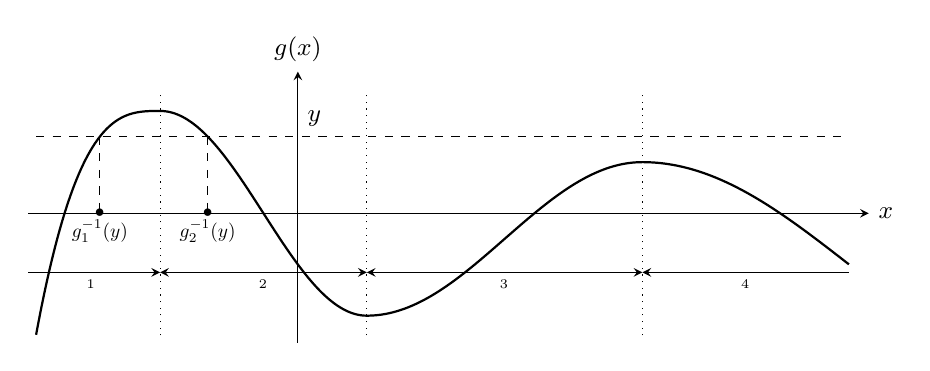
\begin{tikzpicture}%[scale=.9]
\shorthandoff{>}
%
\pgfmathsetmacro{\sx}{1.75};% x-scaling
%
% transformacion g' = 0 medida nula
\begin{scope}
%
\pgfmathsetmacro{\sy}{1.3};% y-scaling 
%
\draw[>=stealth,->] ({-1.9*\sx-.1},0)--({\sx*4+.25},0) node[right]{\small $x$};
\draw[>=stealth,->] (0,{\sy*(-3*.9^3+1)-.1})--(0,{\sy+.5}) node[above]{\small $g(x)$};
%
\draw[thick]
plot[domain=-1.9:-1,samples=100] ({\sx*\x},{\sy*(3*(\x+1)^3+1)})
-- plot[domain=-1:.5,samples=100] ({\sx*\x},{\sy*cos(120*(\x+1))})
-- plot[domain=.5:2.5,samples=100] ({\sx*\x},{\sy*(.75*sin(90*(\x-1.5))-.25)})
-- plot[domain=2.5:4,samples=100] ({\sx*\x},{\sy*(cos(60*(\x-2.5))-.5)})
;
%
\draw[dashed] ({-1.9*\sx},{.75*\sy})--({4*\sx},{.75*\sy});
\draw (0,{.75*\sy}) node[above right]{\small $y$};
%
\draw[dashed] ({-\sx*(1+(.25/3)^(1/3))},{.75*\sy})--({-\sx*(1+(.25/3)^(1/3))},0)
node[scale=.7]{$\bullet$} node[below,scale=.7]{$g_1^{-1}(y)$};
%
\draw[dashed] ({\sx*(acos(.75)/120-1)},{.75*\sy})--({\sx*(acos(.75)/120-1)},0)
node[scale=.7]{$\bullet$} node[below,scale=.7]{$g_2^{-1}(y)$};
%
%
\draw[dotted] ({-\sx},{-\sy-.25})--({-\sx},{\sy+.25});
\draw[>=stealth,->] ({-\sx*1.9-.1},-.75)--({-\sx},-.75);
\draw ({-1.5*\sx},-.75) node[below,scale=.8]{\small $\X_1$};
%
\draw[dotted] ({.5*\sx},{-\sy-.25})--({.5*\sx},{\sy+.25});
\draw[>=stealth,<->] ({-\sx},-.75)--({.5*\sx},-.75);
\draw ({-.25*\sx},-.75) node[below,scale=.8]{\small $\X_2$};
%
\draw[dotted] ({2.5*\sx},{-\sy-.25})--({2.5*\sx},{\sy+.25});
\draw[>=stealth,<->] ({.5*\sx},-.75)--({2.5*\sx},-.75);
\draw ({1.5*\sx},-.75) node[below,scale=.8]{\small $\X_3$};
%
\draw[>=stealth,<-] ({2.5*\sx},-.75)--({4*\sx},-.75);
\draw ({3.25*\sx},-.75) node[below,scale=.8]{\small $\X_4$};
\end{scope}
%
%
% % reparticion
% \begin{scope}[xshift=8.5cm]
% %
% \pgfmathsetmacro{\sy}{2};% y-scaling 
% %
% \draw[>=stealth,->] (-.6,0)--({\sx*4+.25},0) node[right]{\small $x$};
% \draw[>=stealth,->] (0,-.25)--(0,{\sy+.5}) node[above]{\small $F_X$};
% %
% \draw[thick] (-.5,0)--(0,0)--(\sx,{\sy/2})--({2*\sx},{\sy/2})
% -- plot[domain=2:3,samples=100] ({\sx*\x},{\sy*(1+(\x-2)^(3/2))/2})
% -- ({\sx*4},\sy);
% %
% \draw (\sx,0)--(\sx,-.1) node[below,scale=.9]{\small $1$};
% \draw ({2*\sx},0)--({2*\sx},-.1) node[below,scale=.9]{\small $2$};
% \draw ({3*\sx},0)--({3*\sx},-.1) node[below,scale=.9]{\small $3$};
% \draw (\sx,0)--(\sx,-.1) node[below,scale=.9]{\small $1$};
% %
% \draw (0,{\sy/2})--(-.1,{\sy/2}) node[left,scale=.7]{\small $1/2$};
% \draw (0,\sy)--(-.1,\sy) node[left,scale=.7]{\small $1$};
% %
% \draw ({\sx*2.25},-1) node{\small (b)};
% \end{scope}
%
\end{tikzpicture} \end{center}
%
\leyenda{\modif{(a): Ilustraci\'on de una transformaci\'on $g$ no inyectiva, tal
    que  $\X_{[0]} =  \{  x,  \: g'(x)  =  0 \}$,  representado  por las  lineas
    punteadas  ($x$  correspondiente),  es  de  medida de  Lebesgue  nula.   Los
    $\X_{[k]}$ son descrito debajo de  cada dominio.  La linea discontinua da un
    nivel $y$  y los  puntos en el  eje $x$  representan $g_k^{-1}(y), \:  k \in
    I(y)$; en el ejemplo, $I(y) = \{ 1 \,  ; \, 2 \}$ \ y, suponiendo de que $\X
    = \Rset$, \ $F_Y(y) = F_X(g_1^{-1}(y)) + 1-F_X(g_2^{-1}(y))$.}}
\label{fig:MP:TransformacionVA}
\end{figure}

\modif{Una tercera alternativa,  a pesar que sea delicado,  es de apoyarse sobre
  la teoria  de las  distribuciones y} expresar  como \ $\displaystyle  p_Y(y) =
\int_\X  p_X(x) \,  \delta(y-g(x)) \,  dx$, donde  se usa  la expansi\'on  de la
funci\'on delta  en t\'erminos  de sus ceros:  \ $\delta(y-g(x)\,)=  \sum_{k \in
  I(y)}    \frac{1}{\left|   g_k'\left(    g_k^{-1}    (y)   \right)    \right|}
\delta(x-g_k^{-1}(y))$~\cite{ManWol95}.

Es  importante  notar  de  que  la  condici\'on $\X_{[0]}$  de  medida  nula  es
importante. El el caso contrario,  $Y$ no queda continua. Por ejemplo, considera
$X$ uniforme sobre  \ $\X = (  3 \, ; \,  3)$ \ y \ $Y  = g(X)$ \ con  \ $g(x) =
\left(  1 + \cos\left(  (|x|-1) \frac{\pi}{2}  \right) \right)  \un_{(1 \,  ; \,
  3)}(|x|) +  2 \un_{[0 \, ;  1]}(|x|)$.  Esta funci\'on  es representado figura
Fig.~\ref{fig:MP:TransformacionVANoContinua}-(a).    Claramente,  \  $g$   \  es
continua y diferenciable sobre $\X$, pero con \ $\X_{[0]} = [ -2 \, ; \, 1]$ que
no  es  de medida  nula.   Saliendo  de $F_Y(y)  =  P(g(X)  \le  y)$ se  calcula
sencillamente  $F_Y(y)  = \frac23  \left(  1  -  \frac1\pi \arccos(y-1)  \right)
\un_{[0  \,  ; \,  2)}  +  \un_{[ 2  \,  ;  \,  +\infty)}(y)$, ilustrada  figura
Fig.~\ref{fig:MP:TransformacionVANoContinua}-(b).   Claramente   \  $F_Y$  \  es
discontinua en \ $y = 2$: \ $Y$ \ no es continua.

\begin{figure}[h!]
\begin{center} \begin{tikzpicture}%[scale=.9]
\shorthandoff{>}
%
\pgfmathsetmacro{\r}{.05};% radius arc non continuity F_X y/o p_X
%
% transformacion g' = 0 medida no nula
\begin{scope}
%
\draw[>=stealth,->] (-3.6,0)--(3.75,0) node[right]{\small $x$};
\draw[>=stealth,->] (0,-.25)--(0,2.5) node[above]{\small $g(x)$};
%
\draw[thick]
(-3.4,0)--(-3,0)--
plot[domain=-3:-1,samples=100] (\x,{1+cos(90*(1+\x))})--
(1,2)--
plot[domain=1:3,samples=100] (\x,{1+cos(90*(1-\x))})--
(3.5,0);
%
\draw (-3,0)--(-3,-.1) node[below,scale=.8]{\small $-3$};
\draw (-2,0)--(-2,-.1) node[below,scale=.8]{\small $-2$};
\draw (-1,0)--(-1,-.1) node[below,scale=.8]{\small $-1$};
\draw (1,0)--(1,-.1) node[below,scale=.8]{\small $1$};
\draw (2,0)--(2,-.1) node[below,scale=.8]{\small $2$};
\draw (3,0)--(3,-.1) node[below,scale=.8]{\small $3$};
%
\draw (0,1)--(-.1,1) node[left,scale=.8]{\small $1$};
\draw (-.1,2) node[above left,scale=.8]{\small $2$};
%
\draw[>=stealth,<->] (-3,-.5)--(-1,-.5); \draw (-2,-.5) node[below,scale=.9]{\small $\X_{[1]}$};
\draw[>=stealth,<->] (1,-.5)--(3,-.5); \draw (2,-.5) node[below,scale=.9]{\small $\X_{[2]}$};
\draw[>=stealth,<->] (-1,-.5)--(1,-.5); \draw (0,-.5) node[below,scale=.9]{\small $\X_{[0]}$};
%
\draw(0,-1.5) node{\small (a)};
\end{scope}
%
%
% reparticion
\begin{scope}[xshift=7cm]
%
\pgfmathsetmacro{\sx}{1.5};
\pgfmathsetmacro{\sy}{2};% y-scaling 
%
\draw[>=stealth,->] (-.6,0)--({3*\sx+.5},0) node[right]{\small $y$};
\draw[>=stealth,->] (0,-.25)--(0,{\sy+.25}) node[above]{\small $F_Y$};
%
\draw[thick] (-.5,0)--(0,0)--
plot[domain=0:2,samples=250] ({\sx*\x},{\sy*2*(1-acos(\x-1)/180)/3});
%
\draw ({2*\sx+\r},{2*\sy/3+\r}) arc (90:260:\r);
%--
\draw[dotted] ({2*\sx},{2*\sy/3})--({2*\sx},\sy);
\draw[thick] ({2*\sx},\sy) node[scale=.7]{$\bullet$}--({3*\sx},\sy);
%
\draw ({\sx},0)--({\sx},-.1) node[below,scale=.8]{\small $1$};
\draw ({2*\sx},0)--({2*\sx},-.1) node[below,scale=.8]{\small $2$};
\draw ({3*\sx},0)--({3*\sx},-.1) node[below,scale=.8]{\small $3$};
%
\draw (0,{2*\sy/3})--(-.1,{2*\sy/3}) node[left,scale=.7]{\small $2/3$};
\draw (0,\sy)--(-.1,\sy) node[left,scale=.7]{\small $1$};
%
\draw({1.75*\sx},-1.5) node{\small (b)};
\end{scope}
%
\end{tikzpicture} \end{center}
%
\leyenda{\modif{En (a)  se dibuja $g(x) = \left( 1  + \cos\left( (1-|x|) \frac{\pi}{2}
    \right)   \right)   \un_{(1  \,   ;   \,  3)}(|x|)   +   2   \un_{[0  \,   ;
    1]}(|x|)$. Suponiendo de que $\X = (-3 \, ; \, 3)$, claramente $\X_{[0]} = [
  -1 \,  ; \, 1]$ no  es de medida nula,  dando para $X$ uniforme  sobre $\X$ la
  variable $Y = g(X)$ no continua de funci\'on de repartici\'on representenda en
  (b).  }}
\label{fig:MP:TransformacionVANoContinua}
\end{figure}
  }

%Sea $X$ una  variable aleatoria (continua, en general)  definida en el intervalo
%$[x_m, x_M]$ con funci\'on densidad  de probabilidad $p(x)$. Sea $Y=\Psi(X)$ una
%funci\'on real  de $X$, luego $Y$  toma los valores $y=\Psi(x)$  en el intervalo
%$[y_m,y_M]$.  La funci\'on  densidad  de probabilidad  $q(y)$  para la  variable
%aleatoria transformada $Y$ se obtiene  de la siguiente manera, dependiendo de la
%forma de la transformaci\'on:
%
%\begin{itemize}
%\item Si  $\Psi$ es inversible, con  inversa (\'unica), se  tiene \ $x=\Phi(y)$,
%  con  $\Phi=\Psi^{-1}$.  A partir  de  la  propiedad  de conservaci\'on  de  la
%  probabilidad
%  %
%  $$
%  |q(y)\, dy| = |p(x) \, dx|
%  $$ 
%  %
%  para  una correspondencia  biun\'ivoca  entre $x$  e  $y$, se  obtiene la  pdf
%  transformada
%  %
%  $$
%  q(y)  = p(x)  \left| \frac{dx}{dy}  \right| =  p\left(\Phi(y)\right)  \ \left|
%    \Phi'(y)   \right|   =  \frac{p\left(\Phi(y)\right)}{\left|   \Psi'(\Phi(y))
%    \right|} .
%  $$
%  %
%  Una forma alternativa  de derivar este resultado es partir  de la funci\'on de
%  repartici\'on:
%  %
%  $$
%  F_Y(y)  =  P(Y\leq  y)  =  P(\Psi(X)  \leq  y)  =  P(X\leq  \Psi^{-1}  (y))  =
%  F_X(\Phi(y))
%  $$
%  %
%  y  calcular las  derivadas del  primer y  \'ultimo t\'erminos  respecto  de la
%  variable transformada~$y$.
%
%\item Si la inversa de $\Psi$  es multivaluada, cada valor de $y$ se corresponde
%  con  un conjunto de  valores de  $x$, digamos  $\{x_k =  \Phi_k(y), \  k=1, 2,
%  \ldots\}$.  Debido a  que  estas soluciones  son  mutuamente excluyentes,  las
%  probabilidades se suman, de modo que
%  %
%  $$
%  q(y)   =    \sum_k   p(x_k)   \left|   \frac{dx_k}{dy}    \right|   =   \sum_k
%  \frac{p\left(\Phi_k(y)\right)}{\left| \Psi'(\Phi_k(y)) \right|} ,
%  $$
%  %
%  que   formalmente  
%\hfill
%
%Consideramos ahora el  caso de un vector aleatorio  $\mathbf{X} = \{X^1, \ldots,
%X^d\}$  con  funci\'on  densidad  de  probabilidad conjunta  \  $p(x^1,  \ldots,
%x^d)$. Se  define otro vector aleatorio  \ $\mathbf{Y} =  \{Y^1, \ldots, Y^d\}$,
%por   medio   de   las   transformaciones  \   $Y^j=\Psi^j(X^1,\ldots,X^d)$,   \
%$j=1,\ldots,d$. Suponiendo que las  funciones $\Psi^j$ tienen inversa (\'unica),
%se  puede escribir \  $X^j=\Phi^j(Y^1,\ldots,Y^d)$ para  cada $j$.  La funci\'on
%densidad de probabilidad conjunta $q(y^1,\ldots,y^d)$ para $\mathbf{Y}$ se puede
%obtener a partir de la propiedad de conservaci\'on de la probabilidad
%%
%$$
%|q(y^1,\ldots,y^d)\ dy^1\cdots dy^d| = |p(x^1,\ldots,x^d) \ dx^1\cdots dx^d| .
%$$ 
%%
%Para  una  correspondencia biun\'ivoca  entre  $\mathbf{x}$  e $\mathbf{y}$,  se
%obtiene la pdf transformada
%%
%$$
%q(y^1,\ldots,y^d) = \left| \Jac_\Phi \right| \, p(x^1,\ldots, x^d) 
%%%= \int  p(x^1,\ldots, x^d) \delta(y^1-\Psi^1) .......  dx^1 .....
%$$
%%
%donde  $\Jac_\Phi =  \frac{\partial(\Phi^1  , \ldots  , \Phi^d)}{\partial(y^1  ,
%  \ldots , y^d)}$ es el Jacobiano de la transformaci\'on.

%% Ejercicio: Estudiar el caso multivaluado / Resolver un ej. 

\

\aver{\SZ{No toque todav\'ia. Se puede hacerlo con vectores. Caso circular\ldots}

\hfill

Una  \emph{variable  aleatoria  compleja}   $Z=X+i  Y$  puede  interpretarse  en
t\'erminos de las  dos variables aleatorias reales $X$ e $Y$.  La pdf asociada \
$P(z)=p(x,y)$ est\'a dada por la  funci\'on densidad de probabilidad conjunta de
las variables reales. La condici\'on de normalizaci\'on se escribe
%
$$
\int P(z) \, d^2 z = 1
$$
%
donde $d^2 z=dx\,dy$.
}


\SZ{Tratar el caso de leyes condicionales; hablar de simulaci\'on? Metoto inverso, mezcla, rejeccion, a traves de la condicional para el caso vectorial?}